% final draft
% todo: Interkapitel-Referenzen, Kontextgrafik

\chapter{Grundlagen der Realisierung und verwandte Arbeiten} % (fold)
\label{cha:implementierung_Überblick}

Zur Umsetzung des Werkzeugs wurde -- wie in Kapitel \ref{cha:anforderungen} gefordert -- ein „Tangible Tabletop Interface“ verwendet. Tabletop Interfaces zeichnen sich im Generellen dadurch aus, dass im Gegensatz zu handelsüblichen Rechnern nicht nur die Software sondern auch die Hardware applikationsspezifisch ist und nicht für beliebige Anwendungen eingesetzt werden kann. Die Hardware bildet dabei einen Teil oder die gesamte Benutzungsschnittstelle sowohl ein- als auch ausgabeseitig ab. Im speziellen Fall eines „Tangible Tabletop Interfaces“ basiert der Benutzerinteraktion auf der Verwendung physischer Bausteine („Tokens“), die auf der physischen Oberfläche des Interfaces manipuliert werden. Diese Interaktionsform wird von Tabletop Interfaces ergänzt, die die Benutzerinteraktion ausschließlich auf Gesten bzw. Berührungen der Oberfläche abbilden (horizontal verbaute „Touch-“ bzw. „Multi-Touch-Displays“).

Tabletop Interfaces wurden Mitte der 1990er-Jahren in den Arbeiten von Ishii \& Ullmer erstmals vorgestellt. Auch die erste Anwendung, die sich mit Modellierung auf Tabletop Interfaces beschäftigt, stammt aus dieser Zeit. Mit dem Fortschreiten der technologischen Entwicklung ist heute ein Status erreicht, in dem mit Hilfe generischer Identifikations-Frameworks schnell und ohne großen Aufwand Applikationen mit „tangiblen“ Eingabekanälen erstellt werden können. Zur Zeit noch im Prototypenstatus befinden sich Systeme, die sich mit Möglichkeiten des tangiblen Informationsoutputs beschäftigt. Der Rückkanal vom Rechner zum Benutzer wird heute zumeist durch die Projektion von Inhalten auf die Arbeitsoberfläche umgesetzt.

In den folgenden Abschnitten wird die historische Entwicklung von Tabletop Interfaces sowie der aktuelle Stand der Entwicklung im Anwendungsbereich dieser Arbeit betrachtet. Es werden dabei die grundlegenden Konzepte und Eigenschaften der jeweiligen Arbeiten betrachtet und das Potential hinsichtlich der Umsetzung von in Kapitel \ref{cha:anforderungen} identifizierten Anforderungen an das hier entwickelte Werkzeug betrachtet. Abbildung \ref{fig:img_Kontextgrafiken_k6} stellt dieses Kapitel und dessen Aufbau im Kontext der anderen inhaltlich vor- und nachgelagerten Kapitel dar.

\begin{figure}[htbp]
	\centering
		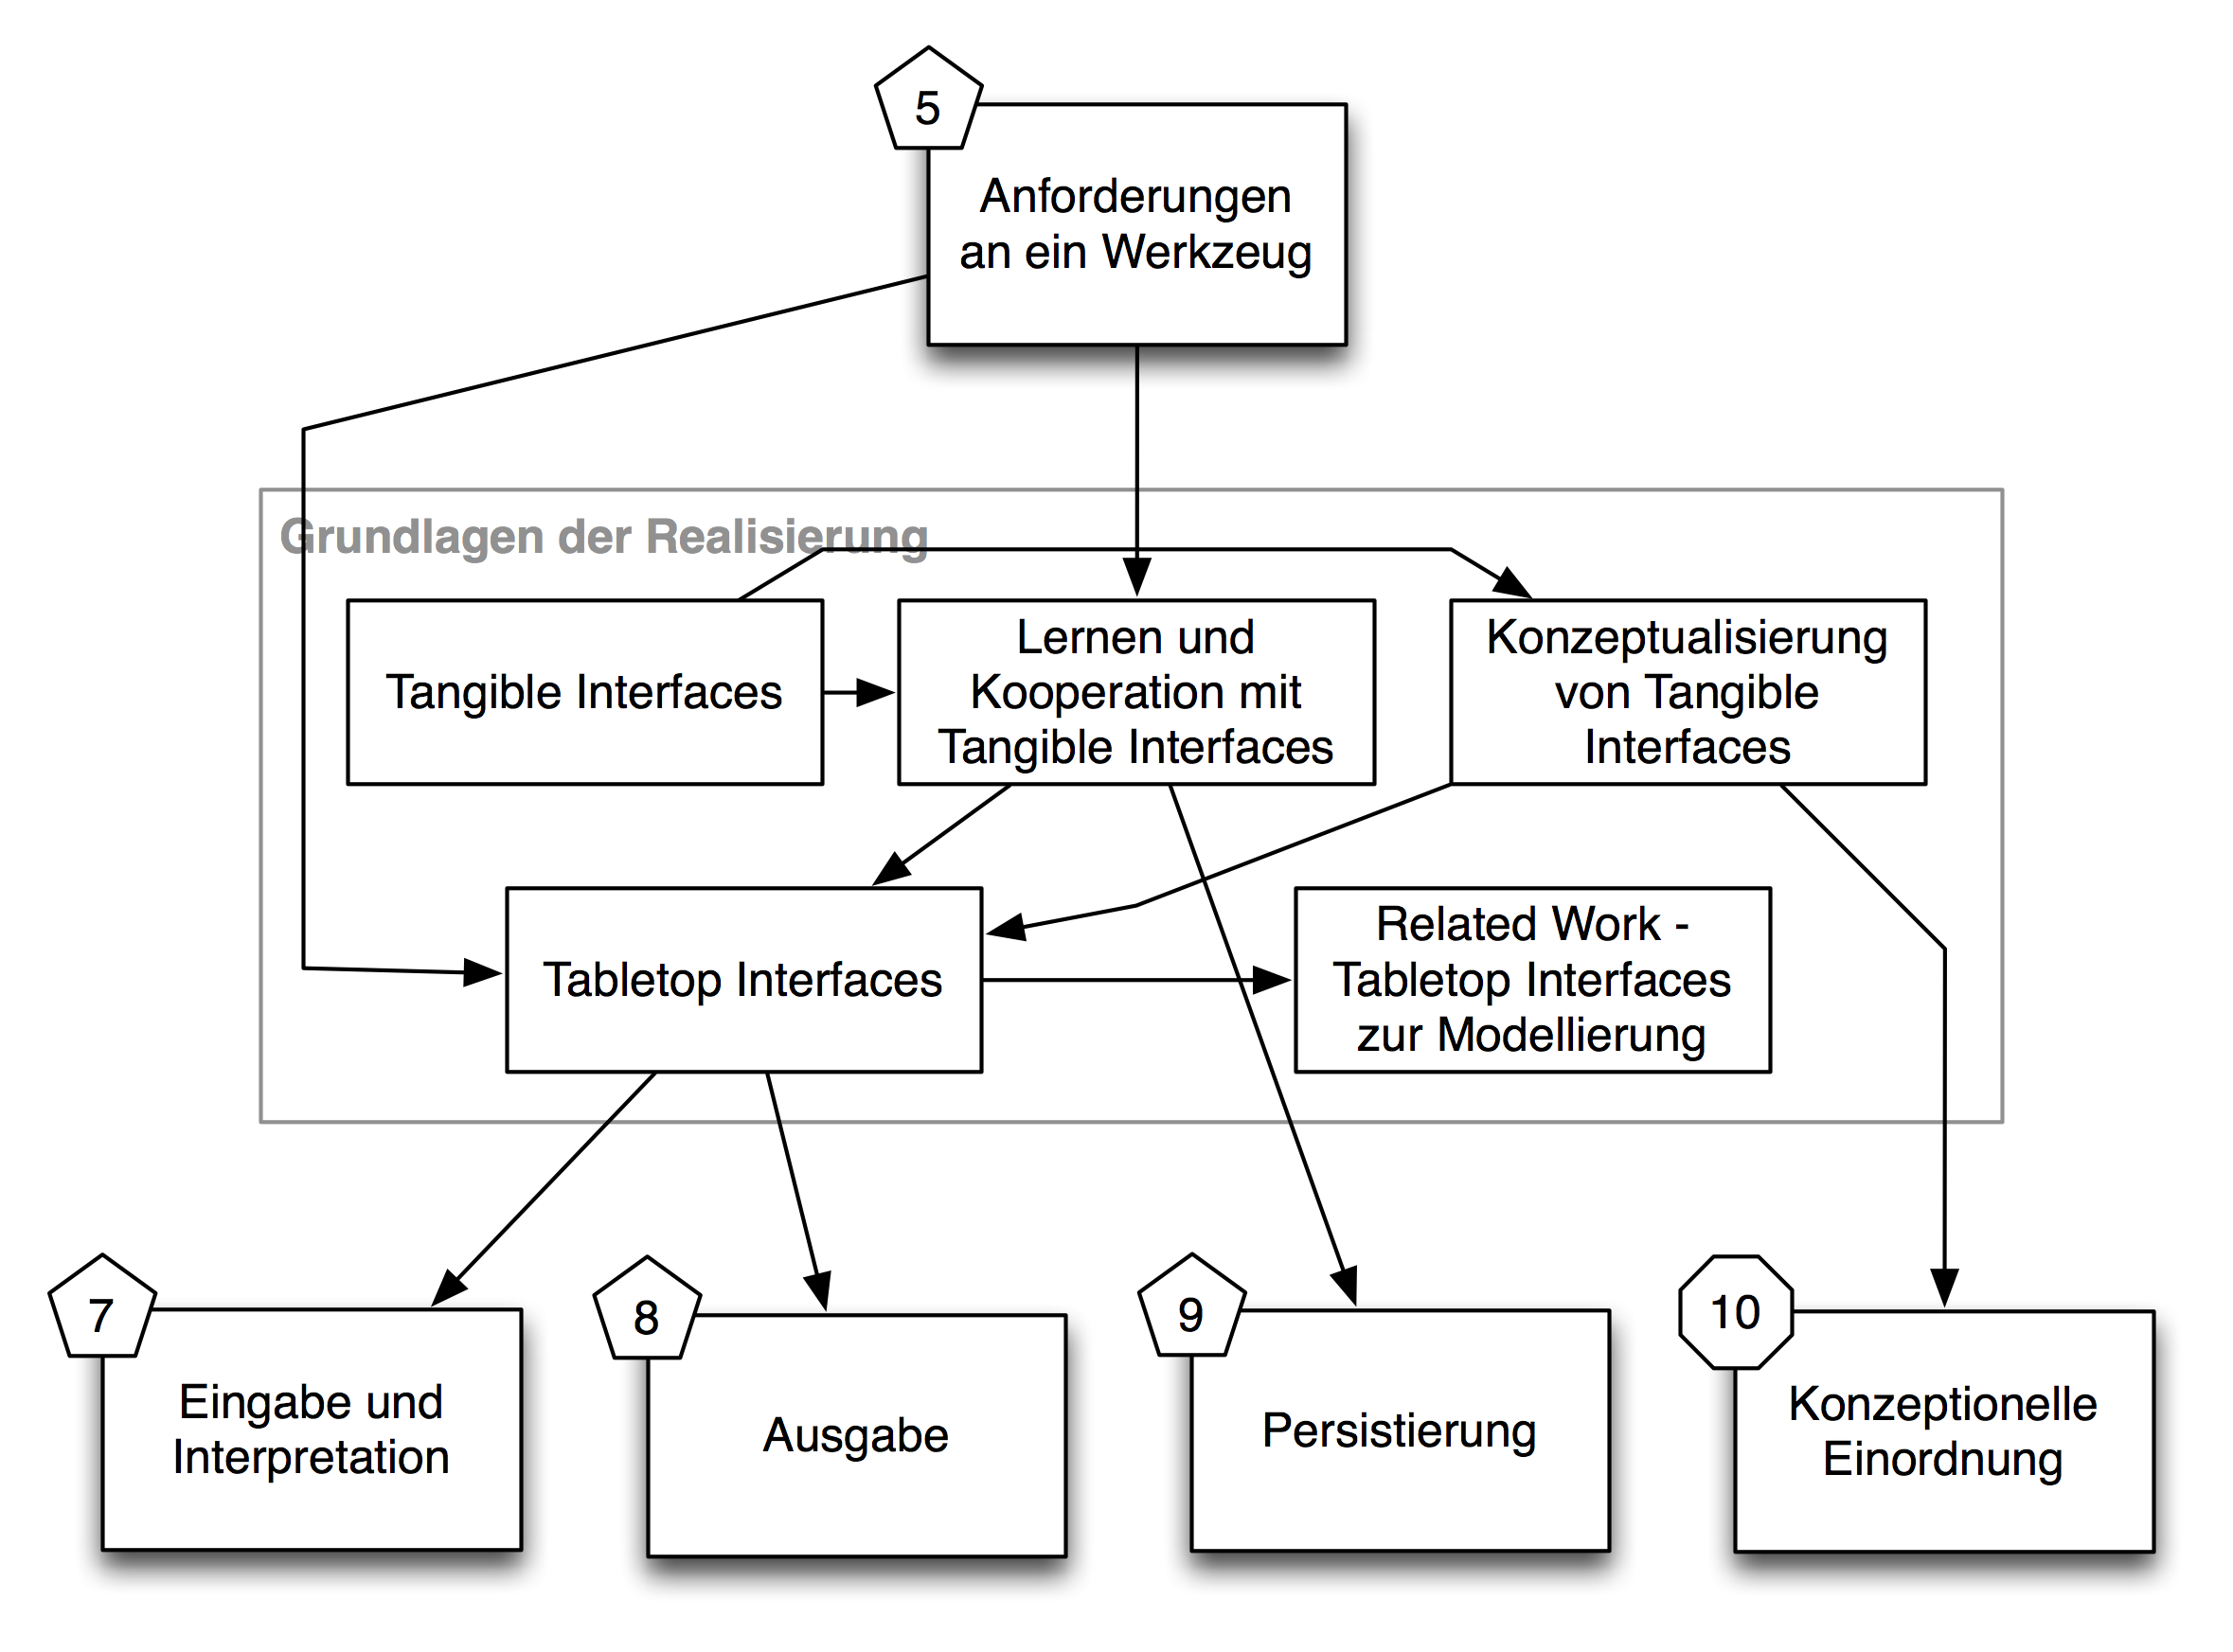
\includegraphics[scale=0.6]{img/Kontextgrafiken/k6.png}
	\caption{Kapitel „Grundlagen der Realisierung und verwandte Arbeiten“ im Gesamtzusammenhang}
	\label{fig:img_Kontextgrafiken_k6}
\end{figure}

\section{Historischer Überblick} % (fold)
\label{sec:entwicklung_tangible_interfaces}

\citet{Wellner93a} und \citet{Suzuki95} werden als jene Arbeiten angesehen, die die Vision von alternativen Benutzungsschnittstellen für Computer maßgeblich geprägt haben. „Alternativ“ bedeutet in diesem Zusammenhang die Verwendung von Ein- und Ausgabekanälen, die sich von den herkömmlichen Werkzeugen wie Tastatur und Maus bzw. Bildschirmen insofern unterscheiden, als dass sie eine unmittelbare Interaktion mit der digital repräsentierten Information ermöglichen und deren Zustand in der realen Welt widerspiegeln.

Der Begriff der „Tangible“ bzw. „Graspable Interfaces“ – also der „berührbaren“ oder „begreifbaren“ Benutzungsschnittstellen — stammt ebenfalls aus der Mitte der neunziger Jahre des zwanzigsten Jahrhunderts. \citet{Fitzmaurice95} werden im Allgemeinen als die Ersten betrachtet, die den Begriff des „Graspable User Interfaces“ prägen und damit die Manipulierbarkeit digitaler Information durch physische Mittel beschreiben. \citet{Fitzmaurice96} präzisiert später den Begriff durch die Abgrenzung zwischen (herkömmlichen, maus-, tastatur- und bildschirmbasierenden) zeitlich gemultiplexten Schnittstellen, bei denen der Informationsaustausch zwischen Benutzer und System über einen Kanal zeitlich hintereinander erfolgt und den (neuartigen, berührbaren) räumlich gemultiplexten Schnittstellen, bei denen mehrere Kanäle gleichzeitig zur Interaktion zwischen Benutzer und System verwendet werden können. 

Der Begriff des „Tangible User Interfaces“ (TUI) wurde kurz danach bzw. parallel dazu von \citet{Ishii97} eingeführt. \citeauthor{Ishii97} verfolgen dabei bei der Definition den umgekehrten Weg und sprechen von einer „Augmentation der realen Welt durch eine Kopplung von digitaler Information and physische Objekte“\footnote{\emph{“augment the real physical world by coupling digital information to everyday physical objects and environments”}\citep{Ishii97}}. 

Die erwähnte Kopplung wurde von Beginn an bidirektional verstanden. Dies bedeutet, dass sowohl der Zustand der realen Welt die digitale Welt beeinflusst als such umgekehrt die digitale Welt auf die reale Welt zurück wirkt. Der Fokus der Entwicklung lag in den ersten zehn Jahren der Entwicklung des Feldes klar auf den erstgenannten Aspekt. Erforscht wurde im Wesentlichen die Manipulation von digitaler Information mittels physischer Werkzeuge, der Zustand der digitalen Welt wurde zumeist ausschließlich dargestellt, beeinflusste aber die reale Welt nicht weiter. Die Kopplung des physischen Zustands der realen Welt an digitale Information (etwa die Veränderung der Form oder Position von physischen Interface-Objekten durch die Ergebnisse einer im Rechner durchgeführten Berechnung) wurde nur in Ausnahmefällen angesprochen (zumeist unter der Bezeichnung „Ambient Interface“ \citep{Gross03}), strukturiert untersucht wurde dieser Aspekt erstmals von \citet{Patten07}. Nach wie vor verzichtet ein Großteil der vorgeschlagenen Systeme auf die automatisierte Manipulation der realen Welt und beschränkt sich auf die Ausgabe der Information über einen optischen Kanal.

Technologisch gründet sich das Gebiet der Tangible Interfaces auf den Entwicklungen im Bereich des Ubiquitous Computing \citep{Weiser91} und der Augmented Reality \citep{Azuma97}. Auch heute ist die Abgrenzung noch eher konzeptuell zu sehen. Die technischen Mittel der Umsetzung sind vor allem hardwareseitig nach wie vor nicht spezifisch den einzelnen Gebieten zuzuordnen, lediglich softwareseitig ist eine Spezialisierung durch die Entwicklung dedizierter Software-Frameworks zu erkennen.

\section{Lernprozesse und Tangible Interfaces} % (fold)
\label{sec:lernprozesse_und_tangible_interface}

Die Anwendungsbereiche von Tangible Interfaces sind historisch breit gestreut, lassen jedoch eine Fokussierung auf die Unterstützung von kreativen und planenden Prozessen erkennen. Ein wichtiger Anwendungsbereich war schon in den ersten Jahren aktiver Forschung das Gebiet der Unterstützung von Lernprozessen \citep{Resnick98}. Zurückgreifend auf die Ideen Pestalozzis, Montessoris \citep{Montessori05} und Piagets \citep{Piaget76} bzw. Papert \citep{Papert00} schlagen \citet{Resnick98} physische Objekte mit Mitteln der IT anzureichern um Spielzeuge (\emph{„digital manipulatives“}) zu schaffen, mit denen Kinder interagieren können und sich so physikalische bzw. systemtheoretische Konzepte spielerisch zu erschließen. Die Objekte fungieren dabei einerseits als Baumaterialien und „Eingabekanal“ für den Rechner, andererseits gleichzeitig auch als „Ausgabe“- bzw. Feedbackkanal über die Wirkung die in der digitalen Welt (etwa in einer Simulation) mit der Eingabekonstellation erzielt wurde. In einer empirischen Studie untersuchen \citet{Price03} die Verwendung von \emph{„Tangibles“} in spielerischen Lernsituationen. Sie identifizieren mehrere positive Effekte, darunter hohe Motivation bei der Interaktion mit dem System und umfassende kooperative Aktivitäten, die durch das System ermöglicht bzw. unterstützt werden. Als prominentes Ergebnis stellen die Autoren die stark ausgeprägte Tendenz zur Reflexion des Spielprozesses und der Erklärung der eigenen Tätigkeiten heraus. Sie setzen dieses Verhalten mit dem von \citet{Schon84} im Kontext von organisationalem Lernen beschriebene Phänomen der \emph{„reflection in action“} gleich. 

Die Erkenntnisse der Entwicklungen und empirischen Untersuchungen in diesem Bereich wurden sowohl in der frühkindlichen Bildung \citep{Zuckerman05} als auch in organisationalen Lernprozessen zur Erhebung und Abstimmung von Strukturen und Abläufen in Unternehmen \citep{Lego02} eingesetzt. Die dort verfolgten Konzepte sind für diese Arbeit insofern von Interesse, als dass Tangible Interfaces dabei zur Modellbildung im engeren Sinne und -- im Falle der organisationalen Anwendung -- auch für „Articulation Work“ im Allgemeinen eingesetzt wurden.

\citet{Marshall07} versucht die möglichen Einflussfaktoren und Wirkungen von Tangible Interfaces auf Lernprozesse zu strukturieren und in einem analytischen Framework zu beschreiben. Er identifiziert sechs Perspektiven und exemplarisch mögliche Ausprägungen, die es erlauben, die Verwendung eines Tangible Interfaces in Lernprozessen strukturiert zu betrachten (siehe Abbildung \ref{fig:img_ImplementierungUeberblick_marshall_tui_learning}). 

\begin{figure}[htbp]
	\centering
		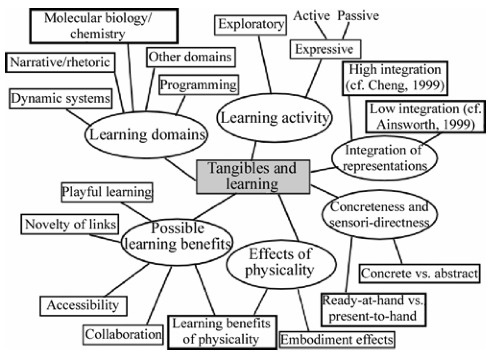
\includegraphics[width=6cm]{img/ImplementierungUeberblick/marshall_tui_learning.png}
	\caption[Tangible Interfaces in Lernprozessen]{Tangible Interfaces in Lernprozessen (entnommen aus \citet{Marshall07})}
	\label{fig:img_ImplementierungUeberblick_marshall_tui_learning}
\end{figure}

Die Perspektive „Learning Domains“ bezieht sich hier auf den Anwendungsbereich des \gls{TUI}. Im konkreten Fall ist diese mit der Arbeits-Domäne, in der die „Articulation Work“ durchgeführt wird, gleichzusetzen und ändert sich deshalb je nach Anwendungsfall.

In der Perspektive „Possible Learning Benefits“ betonen die Autoren mit Bezugnahme auf Arbeiten aus den Kognitionswissenschaften die potentiell positiven Aspekte von physischen Repräsentationen, die durch die haptische Wahrnehmbarkeit verständlicher als rein visuelle Repräsentationen wären. In diesem Zusammenhang erwähnen die Autoren auch die Eignung von Tangible Interfaces in kooperativen Lernsituationen, in denen das Interface durch seine physische Präsenz einen „shared space“ erzeugen würde, in dem Kommunikation und Interaktion erleichtert werden.

Relevant im Kontext von „Articulation Work“ bzw. der Externalisierung und Abstimmung von mentalen Modellen sind die beiden Lernformen, die in der Perspektive „Learning Activity“ identifiziert wurden. Demnach ermöglichen Tangible Interfaces besonders explorative und expressive Aktivitäten. Erstere beziehen sich auf eine Erforschung einer existierenden physischen Repräsentation, die experimentell verändert werden kann und die Entwicklung eines tiefergehenden Verständnisses für das repräsentierte Phänomen ermöglichen würde. Zweitere beziehen sich auf Erzeugung von Repräsentationen mit dem Tangible Interface. Dabei kann die Abbildung direkt erfolgen, alternativ kann aus der Interaktion mit dem Interface eine Repräsentation (etwa eines Arbeitsablaufs) vom System automatisiert abgeleitet werden.

Die übrigen Perspektiven sind für den hier betrachteten Anwendungsfall nur bedingt relevant („Concretness and sensori-directness“) oder werden in späteren Abschnitten noch detaillierter behandelt („Integration of representations“ bzw. „Effects of physicality“). Auf sie wird hier deshalb nicht näher eingegangen.

% section lernprozesse_und_tangible_interface (end)

\section{Kooperation und Tangible Interfaces} % (fold)
\label{sec:kooperation_und_tangible_interfaces}

„Articulation Work“ wird in einem Großteil der Anwendungen kooperativ durchgeführt. Die hier zu unterstützende „explizite Articulation Work“ zur Abstimmung mentaler Modelle mittels Externalisierung findet immer unter Beteiligung mehrerer Individuen statt, die simultan versuchen, ihre individuellen Sichtweisen auf einen Arbeitsablauf abzustimmen. In Kapitel \ref{cha:mentale_modelle} wurde auf die Nützlichkeit von physischen Repräsentationen bei der Externalisierung mentaler Modelle verwiesen. Auch in der Domäne der Tangible Interfaces wurde die Wirkung der dedizierten, physischen Schnittstelle auf die Kooperation der beteiligten Individuen untersucht (erstmals in \citep{Hornecker01}). Die dort gezogenen Schlüsse sind Gegenstand dieses Abschnitts. 

Tangible Interfaces bieten durch die physische Ausgestaltung der Benutzungsschnittstelle oft die Möglichkeit, nicht exklusiven Zugriff auf die Funktionen des Systems und so eine kooperative Verwendung zu ermöglichen. \citet{Hornecker04} geht über die rein simultane Zugreifbarkeit auf das System hinaus und attestiert Tangible Interfaces eine inhärent kooperationsunterstützende Wirkung. Sie identifiziert im Kern vier sozial Effekte von Tangible Interfaces:
\begin{itemize}
	\item Intuitive und simultane Manipulierbarkeit
	\item Fokus-stärkende Wirkung
	\item Awareness, Gestik und perfomative Bedeutung der Handlungen
	\item Externalisierungsfunktion und Rolle als Boundary Object
\end{itemize}

Diese Effekte werden in den folgenden Abschnitten kurz auf Basis der Ausführungen der Autorin zusammengefasst und in den Kontext der Unterstützung von „Articulation Work“ gesetzt. Für eine detaillierte Beschreibung sei hier auf \citep[][S. 147-212]{Hornecker04} verwiesen. Auch die Referenzen zu den einzelnen hier wiedergegebenen Hypothesen sind dort zu finden -- in dieser Arbeit wurde auf deren Angabe verzichtet. 

\subsection{Intuitive und simultane Manipulierbarkeit} % (fold)
\label{sub:intuitive_und_simultane_manipulierbarkeit}

Tangible Interfaces wird eine intuitive Manipulierbarkeit zugeschrieben. Dies bedeutet in diesem Zusammenhang, dass der Zugang zum System spielerisch und erfahrungsorientiert erfolgen kann und keine Übersetzung der intendierten Handlungen auf am Rechner ausführbare Aktivitäten erfolgen muss. Dies ist vor allem für Personen eine Erleichterung, denen der abstahierender Zugang schwerfällt. Konkret zeigt sich das unter anderem bei der Externalisierung von Handlungswissen, das an bestimmte Situationen gebunden ist und von den handelnden Personen nur schwer bzw. nicht generalisiert werden kann. Kann während der Externalisierung in der realen, physischen Welt verblieben werden, erleichtert dies den Zugang zum System und führt im Allgemeinen zu vollständigeren bzw. stimmigeren Externalisierungen.

Zudem ermöglicht ein einfacher Zugang zum System eine Konzentration auf die eigentliche Arbeitsaufgabe -- das Werkzeug tritt in den Hintergrund. Wichtig erscheint in diesem Zusammenhang die Anforderung Änderung einfach rückgängig machen zu können, so dass inhaltliche Experimente einfach und ohne Aufwand korrigiert werden können, wenn sie sich als nicht zielführend erweisen.

Die simultane Manipulierbarkeit vieler Tangible Interfaces fördert ebenfalls die Kooperation bei der Benutzung des Systems. Der nicht-exklusive Zugang zur Benutzungsschnittstelle ermöglicht erst eine unmittelbare Zusammenarbeit am Arbeitsgegenstand. In Kombination mit der intuitiven Manipulierbarkeit wird der Kooperations-Aspekt noch weiter gestärkt, da Spezialkompetenzen zur Bedienung des Systems nicht notwendig sind. Der Zugang zur Schnittstelle wird damit auch egalitärer und schließt nicht einzelne Benutzergruppen von der Bedienung des Werkzeugs aus. Dies wird vor allem in partizipartiven Planungs- und Entwurfsprozessen (wie „expliziter Articulation Work“) deutlich, in denen Personen unterschiedlicher Fach- und Medienkompetenz zusammenarbeiten müssen. 

Der physische Interaktionsraum führt neben der simultanen Manipulierbarkeit auch zu natürlicheren Interaktionsabläufen zwischen den beteiligten Individuen. Im Gegensatz zu Systemen, bei denen im virtuellen Raum interagiert wird, müssen keine expliziten Synchronisationsmechanismen eingeführt werden, die etwa Bearbeitungskonflikte vermeiden. Die Abstimmung erfolgt durch die unmittelbare Manipulation direkt und muss nicht weiter technisch unterstützt werden. Auch ist im Allgemeineren eine feingranularere Interaktion als bei bildschirmbasierter Zusammenarbeit zu beobachten. „Feingranular“ bedeutet hier, dass der Aktivitätsfokus („Turn-taking“) öfter wechselt und somit zu gleichmäßigeren Einzelbeiträgen im Gesamtergebnis führt.

% subsection intuitive_und_simultane_manipulierbarkeit (end)

\subsection{Fokus-stärkende Wirkung} % (fold)
\label{sub:fokus_stärkende_wirkung}

Physische Modelle, die mittel Tangible Interfaces erstellt werden oder Gegenstand desselben sind, wirken nicht nur räumlich fokussierend, sondern konkretisieren auch die inhaltliche Interaktion und fördern lösungsorientierte Diskussionen.

Die inhaltlich fokussierende Wirkung ist auf mehrere Aspekte zurückzuführen, die bei unterschiedlichen Ausprägungen von Tangible Interfaces unterschiedlich stark auftreten. Die folgenden Ausführungen sind im Kontext von (den in dieser Arbeit relevanten) tisch-basierten Systemen zu sehen, auf die sich auch \citet{Hornecker04} vorrangig bezieht.

Der erste erwähnenswerte Einflussfaktor ist die fokussierende Wirkung einer physisch im Zentrum stehenden Repräsentation, die von den beteiligten Individuen „umringt“ wird. Diese Konstellation schafft einen gemeinsamen „Transaktionsraum“ und wirkt als „soziales Signal“ für die Kommunikationsaufnahme. Entfernte (etwa auf eine Wand projizierte) Repräsentationen führen nicht zu derartigen Konstellationen.

Die physische Repräsentation wird zu einem gemeinsamen Bezugspunkt und erzeugt sozialen Druck, sich bei der Diskussion auf sie zu beziehen. Zudem erleichtert sie die Durchsetzung der Forderung nach Konkretisierung von artikulierten Gedanken und visualisiert gleichzeitig die Auswirkungen möglicher Entscheidungen.

Die „Öffentlichkeit“ physischer Repräsentationen, deren Veränderung für alle beteiligten Individuen einsehbar ist, fördert die individuelle Reflexion von eingebrachten Ideen und Gedanken und erleichtert gleichzeitig die Konsensfindung und pragmatische Konfliktlösung.

Wesentliche Faktoren für die fokussierende Wirkung von physischen Repräsentationen sind deren Größe, die Sichtbarkeit und Öffentlichkeit sowie deren Materialiät. Hinsichtlich der Größe existiert sowohl eine Unter- als auch eine Obergrenze für das Auftreten der fokusfördernden Wirkung. Ist die Repräsentation zu klein, ist sie unter Umständen nur für einen Teil der beteiligten Individuen zu erkennen und verhindert eine nicht-exklusive Manipulation. Ist sie zu groß, kann die Repräsentation unter Umständen nicht in ihrer Gesamtheit erfasst werden. 

Neben der Fokuswirkung der Repräsentation ist auch jene der verwendeten Werkzeuge zur Manipulation des Systemzustandes relevant. Im Gegensatz zu generischen Werkzeugen wie Tastatur und Maus schränken physisch für eine bestimmte Aufgabe ausgelegte Werkzeuge den Interaktionsraum auf natürliche Art und Weise ein. Konzeptuell durchdachtes Interaktionsdesign führt so zu einer Fokussierung auf die möglichen Aktionen und lenken die Aufmerksamkeit der Individuen auf jene Strukturen, die durch diese manipuliert werden.

% subsection fokus_stärkende_wirkung (end)

\subsection{Awareness, Gestik und performative Bedeutung der Handlungen} % (fold)
\label{sub:awareness_gestik_und_performative_bedeutung_der_handlungen}

Die physische Präsenz einer Benutzungsschnittstelle im realen Raum erlauben, im Gegensatz zu bildschirmbasierten Schnittstellen, die Aufmerksamkeit nicht ausschließlich auf die Interaktion mit dem System zu konzentrieren. Vielmehr ist es möglich durch die periphäre Wahrnehmung der Umgebung die „Awareness“ \citep{Dourish92} -- also das Bewusstsein über das, was im räumlichen und inhaltlichen Kontext der eigentlichen Aufgabe passiert -- zu erhöhen. 

Die „Awareness“ umfasst auch bzw. vor allem die Tätigkeiten anderer Individuen, die an der Interaktion beteiligt sind\footnote{\emph{„awareness is an understanding of the activities of others, which provides a context for your own activity.“}\citep[][S. 1]{Dourish92}}. Durch die räumliche Nähe sind die Handlungen dieser Individuen nicht nur in ihrer Konsequenz (also der Wirkung auf die Repräsentation) erkennbar, sondern umfassender wahrnehmbar. Handlungen werden schon durch die beginnende Bewegung vor ihrer Durchführung wahrgenommen, auch die eigentliche Handlung erzeugt wahrnehmbare Effekte. Dadurch kommt es zu einer impliziten Abstimmung der Handlungen der einzelnen Personen (gleichzusetzen mit der Durchführung von „implicit Articulation Work“), eine explizite Aushandlung der kooperativen Handhabung der Schnittstelle ist im Normalfall nicht mehr notwendig. Dies korreliert mit der im letzten Abschnitt dargestellten Hypothese, dass physische Benutzungsschnittstellen gegenüber der eigentliche Arbeitsaufgabe in den Hintergrund treten und eine stärke Fokussierung auf diese erlauben.

Das physisch vorhandene Modell fungiert außerdem als Referenzrahmen für non-verbale Kommunikation etwa mittels Gesten. Durch Zeigen auf oder Antippen von Elementen eines \gls{TUI} wird nicht nur der Fokus der Interaktion auf den durch dieses Element repräsentierten Aspekt gelenkt. Je nach Stärke und Ausprägung der referenzierenden Handlung kann damit auch eine performative Bedeutung verbunden sein. So kann zum Beispiel das Weiterreichen eines Elements die Übergabe der Kontrolle ausdrücken oder starkes Antippen eines Elements mit der Aufforderung verknüpft sein dieses in der Diskussion zu berücksichtigen.

% subsection awareness_gestik_und_performative_bedeutung_der_handlungen (end)

\subsection{Externalisierungsfunktion und Rolle als Boundary Object} % (fold)
\label{sub:externalisierungsfunktion_und_rolle_als_boundary_object}

Die Unterstützung von Externalisierung mittels physischer Modelle wurde bereits im Kapitel \ref{cha:mentale_modelle} beschrieben. Tangible Interfaces sind als eben solche Modelle zu verstehen, die eine Schnittstelle zur Manipulation von beliebigen realen oder virtuellen Phänomenen bieten. Wie bereits in Kapitel \ref{cha:mentale_modelle} angeführt, wirken physische Modelle als „Ankerpunkte“ sowohl für individuelle kognitive Vorgänge als auch in der Kommunikation zwischen Individuen.

Die Unterstützung von kognitiven Vorgängen, also der Wirkung von Tangible Interfaces als „Denkhilfe“ ist insofern gegeben, als dass die physische Repräsentation Eingaben dauerhaft abbildet und so verhindert, dass diese im Verlauf der Externalisierung untergehen. Die Repräsentation wirkt so außerdem kummulativ und führt Aspekte zusammen, die in keinem offensichtlichen Zusammenhang stehen. Sie bildet in weiterer Folge auch eine Basis um unter Berücksichtigung aller externalisierten Aspekte Varianten der ursprünglichen Repräsentation zu bilden.  

Externalisierte Repräsentationen wirken auch bei der Kommunikation unterstützend, fungieren in diesem Zusammenhang also als „Sprechhilfe“. Eng in Zusammenhang mit dieser Wirkung steht der Begriff der „Boundary Objects“ \citep{Star89}. „Boundary Objects“ sind Objekte, die der Entwicklung eines gemeinsamen Verständnisses zwischen Individuen aus unterschiedlichen Domänen dienen. Sie bieten im Kern eine fixe, für alle Beteiligten einheitlich verständliche Repräsentation eines beliebigen Phänomens und sind gleichzeitig so flexibel, dass sie in den jeweiligen Domänen mit spezifischer Bedeutung angereichert werden können. Tangible Interfaces wirken -- wenn deren Design offen genug angelegt ist -- als „Boundary Objects“ und erleichtern so die Herausbildung gegenseitigen Verständnisses. In diesem Zusammenhang ist auch die Entstehungshistorie einer physischen Repräsentation von Interesse. Durch die Nachverfolgbarkeit der Entstehung kann das Verständnis der Repräsentation erleichtert werden, da die Herausbildung der im Ergebnis enthaltenen Strukturen nachvollziehbar wird.

% subsection externalisierungsfunktion_und_rolle_als_boundary_object (end)

\subsection{Implikationen} % (fold)
\label{sub:tui_koop_fazit}

Die hier vorgestellten kooperationsfördernden Aspekte von Tangible User Interfaces wurden von \citet{Hornecker04} im Rahmen ihrer Dissertation aus der Literatur identifiziert und empirisch überprüft. Bereits aus der obigen Zusammenfassung wird erkennbar, das ein Großteil der identifizierten Aspekte für „Articulation Work“ im Allgemeinen und die Externalisierung und Abstimmung von mentalen Modellen im Speziellen relevant ist.

Obwohl \citet{Hornecker04} keine Anforderungen an das Design von Tangible Interfaces identifiziert, deren Beachtung zu einer kooperationsfördernden Wirkung führt, können jedoch aus den theoretischen Ausführungen Hinwiese abgeleitet werden, wie ein \gls{TUI} konzipiert werden muss:
\begin{itemize}
	\item Die physische Repräsentation muss räumlich und technisch egalitär zugänglich sein. Das Werkzeug darf die Interaktion zwischen den Benutzern nicht einschränken oder behindern.
	\item Die Größe der Benutzungsschnittstelle muss so ausgelegt sein, dass sowohl eine simultane Manipulierbarkeit der gesamten Repräsentation als auch deren individuelle Erfassbarkeit für alle beteiligten Individuen gegeben ist.
	\item Die Elemente des Tangible Interfaces müssen so konkret sein, dass die Benutzer ihnen eindeutig Bedeutung zuweisen können, gleichzeitig aber offen, dass sie als „Boundary Objects“ zwischen Benutzern aus unterschiedlichen Fachdomänen fungieren können.
	\item Änderungen müssen ohne bleibende Konsequenzen durchgeführt werden können bzw. leicht rückgängig gemacht werden können.
	\item Eine Nachverfolgbarkeit der Entstehungshistorie (ggf. mit Identifikation der individuellen Beiträge) kann zur Verständnisbildung beitragen.	
	
\end{itemize}

% subsection zusammenfassung (end)

% section kooperation_und_tangible_interfaces (end)

\section{Konzeptualisierung und Klassifikation von Tangible Interfaces} % (fold)
\label{sec:konzeptualisierungen_von_tangible_interfaces}

Die Entwicklung des Forschungsgebiets der „Tangible Interfaces“ wurde von mehreren konzeptuellen Arbeiten maßgeblich beeinflusst. Die dort vorgeschlagenen Erklärungsmodelle definieren das Gebiet und grenzen es gegenüber anderen Forschungsbereichen ab. Sie dienen außerdem als Grundlage für die strukturierte Betrachtung und Konzeption konkreter Tangible Interfaces. Im Folgenden werden diese konzeptuellen Arbeiten beschrieben und auf deren Kontext und Spezifika eingegangen.

Zur strukturierten Betrachtung von Tangible Interfaces ist es außerdem notwendig jene Dimensionen zu identifizieren, an denen sich konkrete Systeme einordnen und unterscheiden lassen. Die Ausprägungen dieser Dimensionen ergeben ein Begriffssystem, das bei der Aufbereitung von unterschiedlichen Tangible Interfaces sowie deren Vergleich helfen kann. Die hier vorgestellten Ansätze tragen verschieden detailliert und von unterschiedlichen Standpunkten aus zu dieser Thematik bei. Sie werden in der Folge strukturiert dargestellt und in Kapitel \ref{cha:konzeptuelle_evaluierung} auf das in dieser Arbeit entwickelte System angewandt um so das System-Design aus konzeptueller Sicht zu reflektieren und potentielle Verbesserungs- und Erweiterungsmöglichkeiten zu identifizieren.

Allgemein ist anzumerken, dass eine Vielzahl von Ausdrücken im sich entwickelnden Forschungsgebiet mehrfach belegt wurden und/oder nicht eindeutig definiert sind. Im Folgenden werden die Ausdrücke der jeweiligen Autoren übernommen. Eine Interpretation bzw. Abbildung auf die Terminologie anderer Autoren wird nur vorgenommen, wo sie im jeweiligen Artikel explizit angeführt wurde. In der Zusammenfassung dieses Abschnitts wird versucht, die unterschiedlichen Terminologien nochmals zusammenzufassen und einen Satz an Ausdrücken festzulegen, der im Folgenden für diese Arbeit Anwendung findet.

Am Ende jeder Beschreibung sind in einer tabellarischen Zusammenfassung jeweils die zentralen Konzepte und Beiträge des Ansatzes angeführt. Die Tabellen weisen einheitlich Einträge zu folgenden Themen auf:
\begin{description}
 \item[Kategorien] von Tangible Interfaces, die im Beitrag identifiziert werden  (inkl. Unterscheidungsmerkmal zur Kategoriebildung).
 \item[Konzepte], die bei der Betrachtung bzw. beim Design eines Tangible User Interfaces zur Anwendung kommen.
 \item[Eigenschaften], die ein Tangible User Interface bzw. dessen Komponenten aufweisen können.
 \item[PD-Brücke]: Aussagen, die der Beitrag zur Natur oder Ausgestaltung der Brücke zwischen physischer und digitaler Welt macht.
\end{description}

Wird in einem Beitrag keine Aussage zu einem oder mehreren dieser Themen gemacht, so ist dies explizit durch „---“ angeführt.

Die Ansätze, die in dieser Betrachtung berücksichtigt wurden, sind in der Reihenfolge der zeitlichen Entstehung angeordnet. Eine Beschreibung und Visualisierung der kausalen Zusammenhänge und Bezugnahmen erfolgt in der Zusammenfassung der Ergebnisse in Abschnitt \ref{sub:tui_konzepte_zusammenfassung}. Bei der Beschreibung der Arbeiten wird nicht auf sämtliche vorgestellten Aspekte eingegangen. Es wird vielmehr auf jene Teile eingegangen, die sich mit der Konzeptualisierung oder Klassifikation von Tangible User Interfaces beschäftigen. Die berücksichtigten Ansätze wurden im Rahmen einer umfassenden Literaturstudie identifiziert und sind im Einzelnen:

%\begin{multicols} {2}
    \begin{itemize}
    	\item Bricks \citep{Fitzmaurice95}
    	\item Graspable User Interfaces \citep{Fitzmaurice96}
    	\item Tangible Bits \citep{Ishii97}
    	\item Containers, Tokens und Tools \citep{Holmquist99}
		\item Tangible Object Meaning \citep{Underkoffler99}
    	\item Das MCRpd Interaktions-Modell \citep{Ullmer00}
    	\item Tokens and Constraints \citep{Ullmer02}
    	\item Degree of Coherence \citep{Koleva03}
    	\item Tokens and Constraints zur Spezifikation \citep{Shaer04}
    	\item Kategorien von \gls{TUI}-Anwendungen \citep{Klemmer04}
    	\item Tangible User Interfaces Taxonomy \citep{Fishkin04}
    	\item Tangible Bits: Beyond Pixels \citep{Ishii08}
    \end{itemize}
%\end{multicols}

\subsection{Bricks} % (fold)
\label{sub:bricks}

Mit „Bricks“ stellen \citet{Fitzmaurice95} das erste als „Graspable User Interface“ bezeichnete System vor. Dieses bildet die Grundlage für weitere Arbeiten der Autoren (z.B. \citet{Fitzmaurice96}), die in der Folge noch behandelt werden (siehe Abschnitt \ref{sub:graspable_user_interfaces}). 

Konzeptuell spannen die Autoren am Ende der Arbeit einen „Design Space“ auf, der mögliche Eigenschaften und Parameter eines Tangible User Interfaces definiert und auch deren möglichen Ausprägungen festlegt. Dabei werden einerseits technische Aspekte des Interfaces abgedeckt, andererseits wird aber auch der Aufbau und die Verwendung des \gls{TUI} berücksichtigt. Die Ausprägungen sind dabei rein beschreibender Natur und werden nicht für eine wie auch immer geartete Bewertung oder Klassifikation genutzt. Das Beschreibungsschema ist stark auf auf Interfaces mit aktiv untereinander kommunizierenden Komponenten („Bricks“) abgestellt, die zur Manipulation einer digitalen Anwendung verwendet werden und auf einer physischen Oberfläche bedient werden. Passive bzw. rein informationstragende Elemente ohne Manipulationsfunktion werden nicht berücksichtigt. Dies liegt in der Natur der von den Autoren entwickelten Anwendung und dem zum Zeitpunkt der Erstellung herrschenden Mangel an alternativen Systemen begründet.

\begin{description}
	\item[Brick's internal ability] Haben die physischen Elemente Mechanismen, die zur Darstellung oder Manipulation von Information benutzt werden können? Diese Mechanismen können physischer oder elektronischer Natur sein. (Mögliche Ausprägungen: „inert“ -- „simple expressions“ -- „smart“) 
	\item[Input \& Output] Welche Eigenschafen der physischen Objekte werden zur Eingabe von Information erfasst bzw. zu Ausgabe verwendet? (Keine Ausprägungen, Aufzählung der Eigenschaften für Input und Output)
	\item[Spatially aware] Kann ein Brick seine Umgebung und/oder andere Bricks wahrnehmen? (Mögliche Ausprägungen: „unaware“ -- „mutually aware“ -- „aware of surroundings“) 
	\item[Communication] Wie kommunizieren Bricks untereinander bzw. mit einer eventuell vorhandenen Hintergrund-Infrastruktur (Mögliche Ausprägungen: „Wireless“ -- „Tethered“ -- „Grid board“)
	\item[Interaction time span] Wie lange dauert eine Interaktion der Benutzer mit dem System bei der Erfüllung einer vorgegebenen Aufgabe? (Mögliche Ausprägungen: „quick (within seconds)“ -- „interaction cache (seconds - minutes)“ -- „long-term (days, months, years)“)
	\item[Bricks in use at same time] Wieviele physische Elemente werden simultan verwendet? (Mögliche Ausprägungen (höhere Werte stehen für Größenordnung): „1“ -- „2“ -- „5-10“ -- „50-100“)
	\item[Function assignment] Wie oft und mittels welchem Vorgehen wird Bricks Funktionalität zugeordnet? (Mögliche Ausprägungen: „permanent“ -- „programmable“ -- „transient“) 
	\item[Interaction representations] Werden physische und virtuelle Objekte gleichzeitig verwendet, um den Systemzustand darzustellen bzw. zu manipulieren? (Mögliche Ausprägungen: „all physical“ -- „mix, physical dominates“ -- „balanced mix“ -- „mix, virtual dominates“ -- „all virtual“)
	\item[Physical \& Virtual layers] Werden physische und virtuelle Interaktions-Schichten separat oder kohärent dargestellt? (Mögliche Ausprägungen: „direct (superimposed)“ -- „indirect (separated)“)
	\item[Bond between physical \& virtual layers] Wie stark sind die physischen mit den virtuellen Objekten gekoppelt? (Mögliche Ausprägungen: „tightly coupled (real time sync)“ -- „loosely coupled (batch sync)“)
	\item[Operating granularity] Wie groß ist der Refenzrahmen für die Interaktion mit den physischen Elementen und wie genau werden die Positionen der Elemente aufgelöst? (Mögliche Ausprägungen: „Desktop (fractions of inches accuracy)“ -- „Room (inch accuracy)“ -- „Building (room accuracy)“)
	\item[Operating surface type] Werden die physischen Elemente auf einer fix vorgegebenen, unveränderlichen Oberfläche verwendet oder kann sich die Oberfläche dynamisch verändern (z.B. Information anzeigen)? (Mögliche Ausprägungen: „static (e.g. paper)“ -- „dynamic (e.g. screen)“)
	\item[Operating surface texture] Welche Auflösung oder Textur besitzt die Arbeitsoberfläche, auf der die physischen Elemente bewegt werden? (Mögliche Ausprägungen: „discrete (e.g. grid board)“ -- „continuous, smooth movement“)
\end{description}

Betrachtungsgegenstand ist bei diesem Ansatz das gesamte \gls{TUI}, auf speziifische Eigenschaften einzelnen Komponenten wird nicht separat eingegangen. Die physischen Elemente (hier „Bricks“) werden nicht im Detail betrachtet, sondern nur hinsichtlich ihrer Verwendung im Gesamtsystem und ihrer technischen Einbindung berücksichtigt.
\\[1em]
\begin{tabular}{| p{3cm} | p{10cm} |}
  \hline
  Kategorien & --- \\ \hline
  Konzepte & Brick \\ \hline
  Eigenschaften & \emph{Gesamtsystem}: Brick's internal ability, Input \& Output, Spatially aware, Communication, Interaction time span, Bricks in use at same time, Function assignment, Interaction representations, Physical \& virtual layers, Bond between physical \& virtual layers, Operating granularity, Operating surface type, Operating surface texture \\ \hline
  PD-Brücke & --- \\ \hline
\end{tabular} 

% subsection bricks (end)

\subsection{Graspable User Interfaces} % (fold)
\label{sub:graspable_user_interfaces}

\citeauthor{Fitzmaurice96} legt in jener Arbeit, in der der Begriff des „Graspable User Inferfaces“ erstmals ausführlich eingeführt wird \citep{Fitzmaurice96}, auch Eigenschaften fest, anhand derer sich die „Graspability“ einer Benutzungsschnittstelle zeigt und beurteilen lässt. Im wesentlichen handelt es sich dabei um einen auf die für die Beurteilung der „Graspability“ relevanten reduzierten Satz an Eigenschaften, die bereits in \citep{Fitzmaurice95} angeführt wurden (siehe Abschnitt \ref{sub:bricks}). Die Beurteilung erfolgt auf einer generischen Skala mit Ausprägungen von „niedrig“ bis „hoch“, wobei „hohe“ Werte in mehreren Eigenschaften auf eher hohe „Graspability“ hinweisen. Die Eigenschaften beziehen sich auf Tangible User Interfaces, die lediglich Werkzeuge zur Manipulation von digitalen Daten besitzen, jedoch keine physische Repräsentation von Information aufweisen. Diese Einschränkung ist wiederum auf die historische Entwicklung des Gebiets und die ersten Versuche GUI-Paradigmen in den physischen Raum zu übersetzten zurückzuführen.

\begin{description}
	\item[Space-multiplexing] Ändern sich die Zuordnungen zwischen physischen Elementen und digitalen Funktionen über die Zeit oder existiert eine permanente Zuordnung? (Mögliche Ausprägungen: kontinuierlich von „transient, always reassign“ -- „permanent, never reassign“)
	\item[Concurrency] Ist die gleichzeitige Ausführung mehrere Operationen mit mehreren physischen Elementen (abhängig oder unabhängig voneinander) möglich und vorgesehen? (Mögliche Ausprägungen: „1“ -- „occasionally 2“ -- „2“ -- „3“ -- „more than 3“)
	\item[Physical form] Lässt sich aus der physischen Form auf die ausgeführte Funktion schließen oder sind die Werkzeuge generisch für unterschiedliche Funktionen verwendbar? (Mögliche Ausprägungen: „generic“ -- „specific“) 
	\item[Spatially aware] Erfasst und berücksichtigt das System die Positionen, Orientierung und/oder Nähe der physischen Objekte bei der Interpretation der Interaktion? (Mögliche Ausprägungen: „unaware“ -- „aware“)
	\item[Spatial reconfigurability] Kann das System in unterschiedlichen physischen Kontexten betrieben werden oder kann es ausschließlich ortsgebunden eingesetzt werden? (Mögliche Ausprägungen (bezogen auf \glspl{TUI} aus einzelnen, handhabbaren Objekten): „permanent location“ -- „stationary“ -- „track“ -- „tethered“ -- „free-ranging (rapid layout)“)
\end{description}

\citeauthor{Fitzmaurice96} stellt mit diesen Eigenschaften ein Framework für die Einordnung eines \gls{TUI} als Gesamtsystem zur Verfügung und geht nicht auf einzelne Komponenten ein. Die Eigenschaften beziehen sich auf das Design des Systems und ignorieren dessen Verhalten. Die ersten beiden und die letzte Eigenschaft sind mit einer kontinuierlichen Skala hinterlegt, \emph{physical form} und \emph{spatially aware} sind binäre Eigenschaften, die entweder gegeben sein können oder nicht.
\\[1em]
\begin{tabular}{| p{3cm} | p{10cm} |}
  \hline
  Kategorien & --- \\ \hline
  Konzepte & --- \\ \hline
  Eigenschaften & \emph{Gesamtsystem}: Space-multiplexing (transient -- permanent), Concurrency (1 -- mehr als 3), Physical form (generic, specific), Spatially aware (unaware, aware), Spatial reconfigurability (permanent location -- free-ranging) \\ \hline
  PD-Brücke & --- \\ \hline
\end{tabular} 

% subsection graspable_user_interfaces (end)

\subsection{Tangible Bits} % (fold)
\label{sub:tangible_bits}

\citet{Ishii97} stellen in ihrer Arbeit die Idee der „Tangible Bits“ vor, die die virtuelle Welt mit der realen Umwelt verknüpfen soll. Dabei wird digitale Information mit realen Objekten oder Phänomenen gekoppelt und so „tangibel“ gemacht. Die Autoren unterscheiden drei grundsätzliche Kernkonzepte, mit Hilfe derer die Idee umgesetzt werden kann:
\begin{description}
	\item[Interactive Surfaces], bei denen beliebige Oberflächen in der realen Welt (etwa Wände oder Schreibtische) zu aktiven Schnittstellen zur virtuellen Welt werden.
	\item[Coupling Bits and Atoms], wo physischen Objekten Information zugeordnet wird, so dass die realen Objekte zu Trägern von und Schnittstellen zu digitaler Information werden.
	\item[Ambient Media], bei deren Einsatz Information über die Umgebung der Benutzer vermittelt wird (z.B. mittels Veränderung der Beleuchtung) ohne die eigentliche Tätigkeit zu unterbrechen. 
\end{description}

Die Autoren ordnen Tangible Bits an die Schnittstelle zwischen den Forschungsgebieten „Ubiquitous Computing“ und „Augmented Reality“ ein. „Ubiquitous Computing“ \citep{Weiser91} beschäftigt sich mit Anwendungen, in denen Computer nicht mehr als als solche wahrnehmbare Werkzeuge eingesetzt werden, sondern in der Umgebung integriert sind und von Benutzern nicht mehr bewusst wahrgenommen, sondern nur noch als Teil der Alltagswelt benutzt werden. Tangible Bits erben von dieser Forschungsrichtung die Idee der physischen, natürlichen Interaktion zwischen Benutzern und Rechner, unterscheiden sich aber insofern, dass nach wie vor ein Interface zur virtuellen Welt vorhanden ist, diese also zum Teil noch bewusst wahrgenommen wird. In diesem Aspekt ähneln Tangible Bits den Ideen, die aus der „Augmented Reality“ Forschung stammen. Augmented Reality beschäftigt sich mit Methoden, die die reale Welt mit digitaler Information nahtlos ergänzen bzw. anreichern. Vor allem im Bereich der Ausgabetechnologien werden bei Tangible Bits viele aus dem „Augmented Reality“-Bereich stammende Konzepte eingesetzt.

Nach dieser grundlegenden Begriffsklärung stellen die Autoren Prototypen vor, die sowohl das Konzept der „Interactive Surfaces“ als auch der „Ambient Media“ umsetzten. Erwähnenswert ist im Zusammenhang mit dieser Arbeit der Prototyp „metaDESK“ \citep{Ullmer97}, eine interaktive Oberfläche in Form eines Tisches, auf der die klassischen Interaktionselemente eines \gls{GUI} in die reale Welt transferiert wurden. Dabei wurden die \gls{GUI}-Elemente auf \gls{TUI}-Elemente abgebildet\footnote{dies stellt im Übrigen die historisch erste Erwähnung des Begriffs „Tangible User Interface“ dar}: 
\begin{itemize}
	\item Windows werden auf „Lenses“ abgebildet, also Linsen, die Information zu realen, physischen Elementen anzeigen.
	\item Icons werden in der physischen Welt als „Phicons“ abgebildet und sind im Wesentlichen phyischen Objekte, die Information repräsentieren.
	\item Menüs werden durch „Trays“ repräsentiert, in denen Phicons an unterschiedlichen Stellen abgelegt werden können, wobei jeweils eine spezifische Operation an die Ablageposition gebunden ist. 
	\item Handles (Elemente zur Manipulation von GUI-Objekten) werden durch „Phandles“ abgebildet. Dies sind im Wesentlichen Phicons, die zur Eigabe von Information verwendet werden können.
	\item Widgets (Kontroll- und Steuerelemente) werden durch „Instruments“ abgebildet, welche Phicons sind, die zur Steuerung der jeweiligen Applikation dienen.
\end{itemize}

Ohne hier weiter auf die Beispiele der Autoren einzugehen, ist doch das den Prototypen zugrunde liegende Designkonzept erwähnenswert, etablierte Metaphern aus der realen oder digitalen Welt für die Benutzerinteraktion zu verwenden. In der Diskussion ihrer Ergebnisse identifizieren die Autoren die Thematik der Metaphern, die die Brücke zwischen realer und virtueller Welt schlagen, als eine der interessantesten offenen Fragen für weitere Forschung auf dem Gebiet. Als Schlussfolgerung ihrer Erfahrungen mit den erstellten Prototypen schlagen sie außerdem vor „optischen“ Metaphern besondere Aufmerksamkeit zu schenken, da diese für den Brückenschlag besonders geeignet wären. 

Als optische Metaphern verwenden die Autoren vor allem Beleuchtung, Schattenwurf und Linsen. Sie bilden diese realen Phänomene auf die Schnittstelle zwischen digitaler und realer Welt ab, so dass z.B. digitale Beleuchtung Information sichtbar macht, die in „unbeleuchteten“ Gebieten fehlt, dass reale Objekte digitale Schatten werfen können und so zusätzliche Information transportieren oder dass eine digitale Linse verwendet wird, um reale Objekt „näher“ zu betrachten und Zusatzinformation einzublenden. Bei der Verwendung von Methaphern wird darauf hingewiesen, dass es wichtig wäre auf ein realitätsgetreues Verhalten der digital augmentierten Artefakte zu achten um eine nahtlose Integration der digitalen Information in die reale Welt zu ermöglichen.
\\[1em]
\begin{tabular}{| p{3cm} | p{10cm} |}
  \hline
  Kategorien & Interactive Surfaces, Coupling Bits and Atoms, Ambient Media (Einordnung nach Anwendungsfall) \\ \hline
  Konzepte & Lenses, Phicons, Tray, Phandles, Instruments \\ \hline
  Eigenschaften & --- \\ \hline
  PD-Brücke & zentraler Aspekt: Verwendung etablierter Metaphern \\ \hline
\end{tabular} 

% subsection tangible_bits (end)

\subsection{Containers, Tokens und Tools} % (fold)
\label{sub:containers_tokens_tools}

\citet{Holmquist99} legen ihre Arbeit als konzeptuelle Betrachtung von interaktiven Systemen an, in denen physische Objekte verwendet werden, um auf digitale Information zuzugreifen bzw. diese zu manipulieren. Das Einteilungsschema, das die Autoren vorschlagen, basiert auf der Art und Weise, in der Information an diese physischen Objekte gebunden ist. Grundsätzlich unterschieden sie zwischen \emph{Containern}, \emph{Tokens} und \emph{Tools}. Eine exakte Abgrenzung bzw. eindeutige Zuordnung zu einer Kategorie ist dabei nicht immer möglich oder sinnvoll.

Der hier vorgestellte Ansatz fokussiert auf die physische Interaktion als Eingabemedium, auf den Aspekt der Informationsausgabe wird nicht eingegangen. Dies ist für das Verständnis der folgenden Beschreibungen im Kontext der späteren historischen Entwicklung wichtig und muss bei der Anwendung dieses Ansatzes berücksichtigt werden. 

\subsubsection{Containers}

Als Container werden all jene Objekte bezeichnet, an die beliebige digitale Information gebunden werden kann. Ein Container ist also ein unspezifisches physisches Objekt in einem Tangible User Interface. Sein Aussehen oder andere physische Eigenschaften lassen keine Aussage über die Art der angebundenen Information bzw. die Information selbst zu. 

Beliebige physische Objekte können als Container agieren, sofern sie die Möglichkeit bieten Information in bzw. auf ihnen abzulegen oder wenn sie durch eine Infrastruktur eindeutig identifizierbar sind, so dass Information an sie gebunden werden kann. Container agieren somit ausschließlich als physische Informationsträger und können verwendet werden um Information zwischen Systemen zu transportieren. 

Ein typisches Beispiel ist die Verwendung eines Füllfederhalters als Container, an den beliebige Information gebunden werden kann, um diese von einem Ort zum anderen transportieren zu können. Der Füllfederhalter steht in keinem direkten Zusammenhang mit der angebundenen Information, aus seinem Erscheinungsbild oder seinen Eigenschaften kann nicht auf die angebundene Information geschlossen werden.

\subsubsection{Tokens}

Tokens sind physische Objekte, deren äußeres Erscheinungsbild bzw. deren Eigenschaften in irgendeiner Weise mit der durch sie repräsentierten Information zusammenhängen. Das physische Objekt und die angebundene Information sind nicht mehr voneinander unabhängig, sondern stehen in einem konzeptuellen Zusammenhang. Die äußere Form oder andere physische Eigenschaften dienen of als Hinweis auf die angebundenen Informationsart oder stehen sogar in Zusammenhang mit der konkret angebundenen Information.

Ein typisches Beispiel für ein Token wäre ein Buch, an das über eine eindeutige Identifikation (etwa ein \gls{RFID}-Tag) der jeweilige Text oder Zusatzmaterial gebunden wird. Das physische Buch steht dabei in direktem Zusammenhang mit der angebundenen digitalen Information.

\subsubsection{Tools}
Tools sind physische Elemente, die nicht Information, sondern Funktionen repräsentieren. Die Anwendung von Tools hat dabei nicht unbedingt physische Auswirkungen, jene digitalen, virtuellen Objekte, auf die das Tool angewandt wird, werden aber entsprechend der Funktion des Tools manipuliert.

Beispiele für Tools sind physische Objekte, die zur Auswahl digitaler Objekte dienen oder Objekte wie Linsen, deren Anwendung zusätzliche Information zu anderen Containern oder Tokens abruft.

\subsubsection{Zugriff auf und Interaktion mit Tokens und Containern}

Der Zugriff auf die Information, die an ein Token oder einen Container gebunden ist, erfolgt über \emph{Information Faucets} (also „Informations-Zapfhähne“ oder „-Armaturen“). Diese Faucets sind aktive Komponenten (im Gegensatz zu Tokens und Containern, die im Allgemeinen passive Komponenten sind, also keine dedizierte Elektronik enthalten). Deren Aufgabe besteht darin, aus Tokens oder Containern, die in deren Reichweite gelangen, die angebundene Information zu extrahieren und auszugeben. Faucets können auch dazu verwendet werden, den Zugriff auf Information einzuschränken. So kann die Ausgabe von Information an eine bestimmte Kombination von Tokens oder Containern gebunden werden oder von einem bestimmten Aufenthaltsort abhängig gemacht werden.

Die Anbindung von Information an ein Token oder einen Container kann ebenfalls eingeschränkt sein, bzw. ist im Fall von Tokens per Definition durch den notwendigen Zusammenhang zwischen physischem Element und Information eingeschränkt. Neben dieser konzeptuell notwendigen Einschränkung können auch weitere Regeln geprüft werden oder z.B. die Bindung zwischen Objekt und Information statisch (d.h. unveränderbar) gespeichert werden. 
\\[1em]
\begin{tabular}{| p{3cm} | p{10cm} |}
  \hline
  Kategorien & --- \\ \hline
  Konzepte & Container, Token, Tool, Faucet \\ \hline
  Eigenschaften & --- \\ \hline
  PD-Brücke & Zugriff auf an physische Elemente gebundene Information nur via Faucets, kein direkter Zugriff vorgesehen \\ \hline
\end{tabular} 

% subsection containers_tokens_tools (end)

\subsection{Tangible Objects Meaning} % (fold)
\label{sub:tangible_objects_meaning}

Im Rahmen der Entwicklung einer „Interactive Surface“ zur Stadtplanung („Urp“) stellen \citet{Underkoffler99} ein Kontinuum von möglichen Bedeutungen bzw. Verwendungszwecken der physischen Objekte eines \gls{TUI} vor. Die Ausprägungen auf der Achse unterscheiden sich in der Stärke der Abstraktion der verwendeten Objekte von ihren Gegenstücken in der realen Welt. Im Zentrum der Achse stehen nicht abstrahierte Objekte, die in Struktur und Verhalten ihren realen Entsprechungen ähneln.
\begin{figure}[htbp]
	\centering
		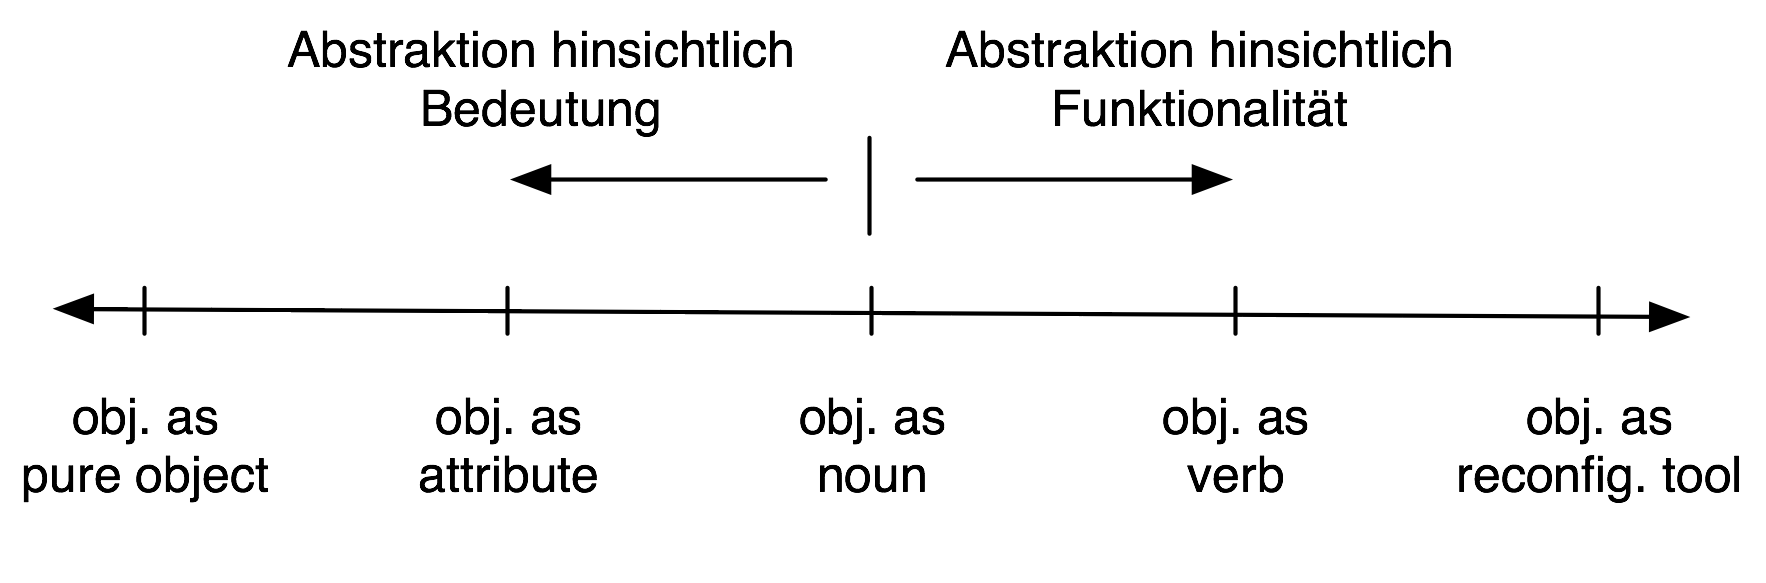
\includegraphics[width=12cm]{img/ImplementierungUeberblick/ObjectMeaning.png}
	\caption[Bedeutung von Objekten in TUIs]{Bedeutung von Objekten in TUIs (adaptiert übernommen aus \citep{Underkoffler99})}
	\label{fig:img_ImplementierungUeberblick_ObjectMeaning}
\end{figure}

\begin{description}
	\item[Object as noun] Derartige Objekte sind Platzhalter für Objekte der realen Welt, denen sie in Form und Verhalten weitgehend entsprechen. Sie stehen für das reale Objekt und werden in dessen Sinne verwendet.
	\item[Object as verb] Die Bedeutung betreffender Objekte reduziert sich auf deren Funktionalität, die Objekte sind nicht mehr Teil der Repräsentation des Systemzustandes sondern werden dazu verwendet, diesen (entsprechend ihrer Funktion) zu verändern.
	\item[Object as reconfigurable tool] Das Objekt wird funktional vollständig von seiner eigentlichen Natur abstrahiert verwendet. Die physischen Eigenschafen stehen nicht mehr in Beziehung zu seiner Verwendung zur Manipulation des Systemzustandes. Die Funktionalität ist dynamisch zuweis- bzw. auswählbar.
	\item[Object as attribute] Objekte werden auf eine ihrer Eigenschaften reduziert. Nur diese wird verwendet, um den Systemzustand abzubilden. Mögliche Eigenschaften sind z.B. Form, Farbe oder Gewicht des Objekts.
	\item[Object as pure Object] Das Objekt wird zum reinen Informationsträger, bei dem die Information nicht in Bezug zur physischen Form oder den Eigenschaften des Objekts steht.
\end{description}

Die Achse ist dabei als konzeptueller Ring zu verstehen, der sich an den beiden Enden wieder schließt. Einem Objekt, dessen physischen Eigenenschaften keine Rolle im \gls{TUI} mehr spielen, kann beliebig Inhalt oder Funktionalität zugewiesen werden, wodurch die Grenze zwischen linkem und rechtem Ende der Achse verschwimmt.
\\[1em]
\begin{tabular}{| p{3cm} | p{10cm} |}
  \hline
  Kategorien & --- \\ \hline
  Konzepte & Object as pure object, Object as attribute, Object as noun, Object as verb, Object as reconfigurable tool  \\ \hline
  Eigenschaften & --- \\ \hline
  PD-Brücke & abhängig von der Art der Tokens  \\ \hline
\end{tabular} 
% subsection tangible_objects_meaning (end)

\subsection{Das MCRpd Interaktions-Modell} % (fold)
\label{sub:mcrpd}

Basierend auf früheren Arbeiten (siehe Abschnitt \ref{sub:tangible_bits}) entwickeln \citet{Ullmer00} ein Modell zur Beschreibung der Interaktion mit Tangible User Interfaces. Es handelt sich bei dieser Arbeit um den ersten Ansatz, der sich diesem Bereich aus Sicht der Systemstruktur nähert und nicht ausschließlich eine reine Klassifikation nach bestimmten Merkmalen eines Systems vornimmt.

Die Autoren grenzen \glspl{TUI} von \glspl{GUI} insofern ab, als das \glspl{TUI} über eine nahtlose Integration zwischen Repräsentation des Systemzustandes und dessen Kontrolle aufweisen (im Gegensatz zu \glspl{GUI}, bei denen der Systemzustand über einen graphischen Kanal ausgegeben wird und über andere Kanäle, etwa Tastatur und Maus, kontrolliert wird). Mit der Forderung nach nahtloser Integration von Repräsentation und Kontrolle -- also im Wesentlichen einer Einheit von Eingabe- und Ausgabe-Kanälen -- wird ein eher striktes Verständnis von \glspl{TUI} vorgeschlagen. Als Tangible User Interface kann ein System demnach nur bezeichnet werden, wenn es Ein- und Ausgabe kohärent über einen Kanal führt.


\begin{figure}[htbp]
	\centering
		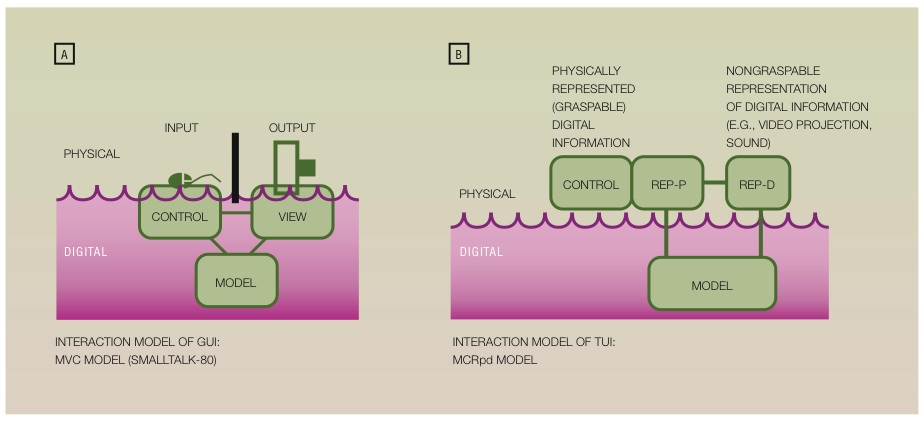
\includegraphics[width=12cm]{img/ImplementierungUeberblick/MCRpd.jpg}
	\caption[Interaktionsmodelle für GUI und TUI]{Interaktionsmodelle für GUI und TUI (übernommen von \citet{Ullmer00})}
	\label{fig:img_ImplementierungUeberblick_MCRpd}
\end{figure}

Diese Verständnis setzten die Autoren in der Folge in einem Interaktionsmodell für \glspl{TUI} um, dass die Struktur eines Tangible User Interfaces konzeptuell beschreibt. Das Modell wird dabei analog zum \gls{MVC}-Modell konzipiert, in dem „View“ und „Controller“ strikt getrennt betrachtet werden. Entsprechend der engeren Kopplung zwischen Repräsentation und Kontrolle wird die Bezeichnung \gls{MCRpd}-Modell vorgeschlagen (siehe Abbildung \ref{fig:img_ImplementierungUeberblick_MCRpd}). Anhand der Gegenüberstellung zwischen \gls{MVC}- und \gls{MCRpd}-Modell wird die Unterscheidung zwischen \gls{GUI} und \gls{TUI} deutlich. Beiden Ansätzen ist gemein, dass der Systemzustand im Rechner durch ein \emph{Model} dargestellt wird. Unterschiede zeigen sich in der Art der Manipulation und Manifestation dieses \emph{Models}. Bei \glspl{GUI} ist Eingabe und Ausgabe strikt getrennt. Die Manipulation des Systemzustandes erfolgt durch die Komponente \emph{Control}, in der physische Kontrollgeräte eine Veränderung des Zustandes erlauben. Die Kontrollgeräte sind dabei im Allgemeinen generisch, d.h. unabhängig vom konkreten Anwendungsfall (also etwa Maus oder Tastatur). Erst durch digitale Kontroll-Elemente wird die Ein- und Ausgabe applikationsspezifisch angepasst. Die Ausgabe erfolgt durch die Komponente \emph{View}, wobei auch in diesem Fall ein generisches Ausgabegerät (etwa ein Bildschirm) verwendet wird. Im Falle eines \gls{TUI} existiert keine Trennung zwischen Ein- und Ausgabe. Das \emph{Model} manifestiert sich durch eine \emph{Representation} in der realen Welt. Diese \emph{Representation} hat eine physische Komponente (\emph{REP-P}) und eine digitale Komponente (\emph{REP-D}), die miteinander verknüpft sind. Die digitale Komponente der Repräsentation umfasst dabei all jene Information, die nicht durch physische, berührbare Elemente dargestellte wird (etwa Projektion, Audio, \ldots). Sie steht dabei jedoch nicht für sich selbst sondern ist immer von eine physischen Repräsentations-Komponente abhängig bzw. dieser zugeordnet. Die physischen Komponenten (\emph{REP-P}) spielen insofern eine zentrale Rolle, als dass ihnen auch die \emph{Control} zugeordnet ist und über sie damit der Systemzustand manipuliert werden kann. Die physischen Komponenten des Ausgabe-Kanals fungieren also zugleich als Instanzen des Eingabe-Kanals.

Basierend auf diesem Ansatz identifizieren die Autoren vier Kern-Charakteristika von Tangible User Interfaces, die sich jeweils an den physischen Komponenten zeigen:
\begin{itemize}
	\item Physikalische Repräsentationen sind mit digitaler Information gekoppelt
	\item Physikalische Repräsentationen enthalten Mechanismen zur Kontrolle des Systems
	\item Physikalische Repräsentationen sind in der Wahrnehmung der Benutzer mit digitalen Repräsentationen gekoppelt
	\item Der physische Zustand eines Tangible Interfaces stellt die Kernaspekt des Systemzustandes dar
\end{itemize}

Aufbauend auf diesen Eigenschaften entwickeln die Autoren in der Folge ein Schema, das unterschiedliche Ansätze bei der Konzeption eines Tangible Interfaces abdeckt. Als zentrale Ansätze werden „spatial“ (räumliche), „relational“ (relationale) und „constructive“ (konstruierende) Ansätze unterschieden. Räumliche Ansätze nutzen die Anordnung der physischen Elemente in einem Referenzrahmen um den Systemzustand zu repräsentieren bzw. zu manipulieren. Bei relationalen Ansätzen ist die räumliche Anordnung unwesentlich, lediglich die Beziehungen zwischen den Elementen codieren den Systemzustand. Konstruierende Ansätze sind zwischen den beiden erstgenannten Ansätzen einzuordnen, da sie Beziehungen zwischen Elementen durch eine räumliche Anordnung der Elemente zueinander abbilden. Systeme, in denen Information lediglich in der Zuordnung zu einem physischen Element codiert wird und nicht in der Beziehung zwischen den Elementen, werden in die Kategorie der „associative“ (assoziativen) Ansätze eingeordnet.

Als zusätzliche Gestaltungsdimension führen die Autoren die Konzeption der physischen Repräsentationen an, die bereits von \citet{Ullmer97} eingeführt wurde. Unterschieden wird hier zwischen „iconic“ und „symbolic representations“, wobei ikonische Elemente einen Bezug zu dem jeweils repräsentierten Objekt der realen Welt haben (etwa ein Bild einer Person), während diese Möglichkeit der Zuordnung bei symbolischen Elementen nicht gegeben ist (etwa bei der Repräsentation einer Person durch ein rotes Rechteck). Aus einer umfassenden Betrachtung der zum Zeitpunkt der Erstellung des Artikels verfügbaren Tangible User Interfaces schließen die Autoren, dass ikonische Repräsentationen vorrangig in räumlichen und assoziativen Ansätzen zum Einsatz kommen, während symbolische Repräsentationen eher bei relationen oder konstruierenden Ansätzen anzutreffen sind.
\\[1em]
\begin{tabular}{| p{3cm} | p{10cm} |}
  \hline
  Kategorien & spatial, relational, constructive, associative (Einordnung nach Art der Informationsrepräsentation)  \\ \hline
  Konzepte & Model, Rep-P, Rep-D, Control \\ \hline
  Eigenschaften & \emph{Rep-P}: iconic, symbolic \\ \hline
  PD-Brücke & Informationsrepräsentation immer an ein physisches Objekt gebunden. Manipulation der Information erfolgt mittels dem gleichen Objekt \\ \hline
\end{tabular} 

% subsection mcrpd (end)

\subsection{Tokens und Constraints nach Ullmer} % (fold)
\label{sub:tokens_und_constraints_nach_ullmer}

Der Token+Constraint-Ansatz wurde von \citet{Ullmer02} erstmals vorgestellt und \citet{Ullmer05} aktualisiert veröffentlicht. \citeauthor{Ullmer05} gehen dabei erstmals von dem Grundsatz aus, dass ein \gls{TUI} zwei grundlegende Arten von physischen Komponenten enthält: Objekte, die digitale Information repräsentieren und Objekte, die die Interaktion mit Computersystemen bzw. die Manipulation des Systemzustands ermöglichen.

In ihren weiteren Ausführungen identifizieren die Autoren zwei grundlegende Arten von \glspl{TUI}, die sich historisch herausgebildet hätten. Einerseits existieren „interactive surfaces“, bei denen physische Objekte benutzt werden um Information auf einer aktiven Oberfläche (zumeist projiziert oder durch einen Bildschirm realisiert) zu manipulieren. Andererseits werden „constructive assemblies“ genannt, deren physische Objekte ohne umgebende Infrastruktur ausschließlich durch reale oder logische Verbindungen zwischen ihnen den Systemzustand ausdrücken. Die Autoren definieren nun eine dritte Art von Systemen und platzieren diese konzeptuell zwischen den beiden zuvor genannten Kategorien. Mit „tokens and constraints“ werden Systeme mit zwei unterschiedlichen Arten von physischen Elementen eingeführt. „Tokens“ stehen für Objekte, die digitale Information repräsentieren. „Constraints“ werden verwendet um (digitale) Funktionalität auf diese Tokens anzuwenden (siehe Abbildung \ref{fig:img_ImplementierungUeberblick_is_tac_ca}).

\begin{figure}[htbp]
	\centering
		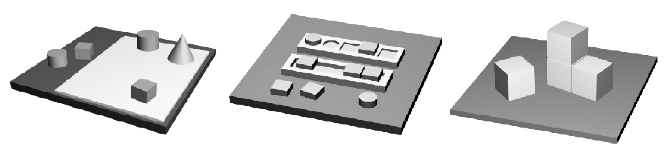
\includegraphics[width=10cm]{img/ImplementierungUeberblick/is_tac_ca.png}
	\caption[Arten von Tangible User Interfaces]{Arten von Tangible User Interfaces -- von links nach rechts: interactive surfaces, tokens+constraints, constructive assemblies (übernommen aus \citet{Ullmer05})}
	\label{fig:img_ImplementierungUeberblick_is_tac_ca}
\end{figure}

In der Folge beschreiben \citeauthor{Ullmer05} die Details des Tokens+Constraints-Ansatzes. Sie gehen dabei zuerst auf die Benutzer-Interaktion in einem Tokens+Constrains-basieren System ein. Diese ist immer in zwei Phasen unterteilt, wobei in der ersten Phase „associate“ Tokens einem oder mehreren Constraints zugeordnet werden. In der zweiten Phase „manipulate“ werden die Tokens im Kontext der Constraints manipuliert, wodurch die digitalen Daten, die an das Token gebunden sind, geändert werden.

Danach widmen sich die Autoren der Abbildung digitaler Information bzw. deren Manipulation auf physische Elemente und definieren vier grundlegende Arten von Beziehungen, die Information abbilden sein können:
\begin{itemize}
	\item die absolute Position eines Tokens in Bezug zu einem Constraint
	\item die relative Position eines Tokens in Bezug zu einem Constraint
	\item die absolute Position eines Tokens in Bezug zu anderen Tokens
	\item die relative Position eines Tokens in Bezug zu anderen Tokens
\end{itemize}
Unter „Position“ sind dabei auch andere spatiale Parameter eines Tokens (wie die Orientierung) zu verstehen.

Nach einer Reihe von Betrachtungen der konzeptuellen Hintergründe und Beispielen kommen die Autoren zu einem weiteren relevanten Punkt, in dem Sie ausführen, wie bzw. warum Tangible Interfaces für Benutzer leichter verständlich sein können als traditionelle \gls{GUI}-basierte Systeme. Bezugnehmend auf \citet{Bellotti02} versuchen Sie Antworten auf fünf von diesen Autoren gestellten Fragen zu finden, die für jede Benutzungsschnittstelle geklärt werden müssen. An dieser Stelle stehen nun nicht die Antworten von \citeauthor{Ullmer05} im Mittelpunkt des Interesses, sondern die Fragen, die einen konzeptuellen Rahmen für das Design einer Benutzungsschnittstelle liefern. Die Fragen stammen aus der Arbeit von \citet{Bellotti02}:
\begin{description}
	\item[Address] Wie weiß das System, dass Benutzer mit ihm und nicht mit anderen (Systemen oder Personen) interagiert?
	\item[Attention] Wie bemerken Benutzer, wenn das System auf eine Interaktionsanforderung reagiert? 
	\item[Action] Wie weiß das System, welchem Objekt der Befehl der Benutzer gilt?
	\item[Alignment] Wie wissen Benutzer, dass das System ihren Befehl korrekt verstanden und ausgeführt hat?
	\item[Accident] Wie werden Missverständnisse zwischen den Benutzern und dem System aufgelöst?
\end{description}
\citeauthor{Ullmer05} beantworten diese Fragen für den Tokens+Constraints-Ansatz jeweils aus konzeptueller und technologischer Sicht. 

Am Ende des Artikels geben die Autoren Varianten des Token+Constraints-Ansatzes an. Durch die Festlegung auf die notwendige Physikalität von Tokens und Constraints ist der Design-Raum eingeschränkt, obwohl die konzeptuellen Überlegungen auch breitere Anwendung finden können. Aus diesem Grund variieren die Autoren ihren Ansatz und geben Alternativen an, die den Grundüberlegungen entsprechen aber unter Umständen nicht alle Vorteile des Kernansatzes aufweisen:
\begin{itemize}
	\item Verwendung von visuellen, graphischen Constraints und physischen Tokens
	\item Verwendung von physischen Constraints für graphische Token
	\item Verwendung von physischen Constraints für nicht-massive Tokens (z.B. Flüssigkeiten)
	\item Verwendung von Tokens und Constraints in durch die Benutzer anpassbaren Größen
	\item Alternative Semantik bei der Abbildung zwischen physischer und digitaler Welt
\end{itemize}

Abschließend wird betont, dass ausgereifte \glspl{TUI} selten in „Reinform“ auftreten, d.h. dass sie nicht exakt einer Kategorie wie „interactive surface“ oder „tokens+constraints“ zugeordnet werden können. 
\\[1em]
\begin{tabular}{| p{3cm} | p{10cm} |}
  \hline
  Kategorien & interactive surfaces, tokens+constraints, constructive assemblies \\ \hline
  Konzepte & Tokens, Constraints \\ \hline
  Eigenschaften & \emph{Token}: Form, absolute und relative Position in Bezug zu Constraints oder anderen Tokens \\ \hline
  PD-Brücke & Codiert in Tokens und in den Beziehungen zwischen Tokens und Constraints \\ \hline
\end{tabular} 

% subsection tokens_und_constraints_nach_ullmer (end)

\subsection{Degree of Coherence} % (fold)
\label{sub:degree_of_coherence}
\citet{Koleva03} schlagen ein Framework vor, dass die Klassifikation von Tangible Interfaces ermöglicht und so das Verständnis der möglichen Verknüpfungen zwischen physischer und digitaler Welt vertiefen soll. Im Gegensatz zu dem von \citet{Ullmer00} mit dem MCRpd-Modell vorgeschlagenen relativ strikten Verständnis eines Tangible Interfaces öffnen \citeauthor{Koleva03} den Begriff und definieren eine kontinuierliche Skala von „Tangibility“, die sich am Grad der „Coherence“ (Kohärenz) zwischen realer und digitaler Welt bemisst. Hohe Kohärenz sagt dabei aus, dass das physische Objekt und sein digitales Gegenstück als ein „Ding“ wahrgenommen werden, also nicht voneinander abgrenzbar sind.

Entlang diesem Kontinuum führen die Autoren Kategorien ein, die die typischen Eigenschaften eines Systems im betreffenden Bereich der Skala beschreiben. Diese Kategorien dienen als Einordnungsschema für Elemente von Tangible Interfaces und können als Grundlage einer Gegenüberstellung unterschiedlicher \glspl{TUI} bzw. deren Komponenten dienen. Entlang der Kohärenz-Skala legen die Autoren folgende Kategorien fest, die sich jeweils auf die Bedeutung des physische Objekt für die Benutzungssschnittstelle beziehen (beginnend mit niedriger Kohärenz): 

\begin{description}
	\item[General-purpose tool] Ein Werkzeug, das zur Manipulation verschiedener digitaler Objekte benutzt werden kann und dabei unterschiedliche Operationen auf diesen Objekten auslösen kann.
	\item[Specialized tool] Ein Werkzeug, das eine bestimmte Operation auslöst, diese aber auf unterschiedliche digitale Objekte anwenden kann.
	\item[Identifier] Objekte, die als Referenz auf ein digitales Objekt agieren. Die Referenz ist nicht zwangsweise permanent, sondern kann unter Umständen dynamisch verändert werden.
	\item[Proxy] Objekte, die insofern enger an die digitale Information gekoppelt sind als Identifier, als dass durch sie die digitale Information manipuliert und nicht nur abgerufen werden kann. 
	\item[Projection] Objekte, die so eng an die digitale Repräsentation gebunden sind, dass dessen physische Eigenschaft Information direkt repräsentiert und die Existenz der Information von der Existenz des Objekts abhängig ist.
	\item[Illusion of same objects] Keine Koppelung im engeren Sinne sondern Identität zwischen realem Objekt und digitaler Information. Ist dann gegeben, wenn beide Komponenten ausschließlich gemeinsam auftreten oder für Benutzer nahtlos von der digitalen in die reale Welt und umgekehrt übergehen.
\end{description}

In der Folge detaillieren die Autoren diese Kategorien und identifizieren Eigenschaften, die eine Verknüpfung zwischen realer und digitaler Welt aufweisen kann und an denen sich der Grad an Kohärenz bemisst bzw. an denen er sichtbar wird:

\begin{description}
	\item[Transformation] Beschreibt, wie Manipulationen am realen Objekt in die virtuelle Welt umgesetzt werden. \emph{Literal Mediation} liegt vor, wenn Manipulationen in realer und virtueller Welt analog umgesetzt werden (wenn z.B. eine Bewegung eines Objekts auch in eine Bewegung dessen realer Repräsentation umgesetzt wird). \emph{Transformed Mediation} liegt vor, wenn eine Manipulation eines realen Objekts eine nicht unmittelbar assozierbare Reaktion in der digitalen Welt auslöst (bei der Rotation eines Tokens etwa die Lautstärke eines Audiokanals verändert).
	\item[Sensing of Interaction] Beschreibt, auf welche Parameter eines Objektes der realen Welt die digitale Repräsentation reagiert. Die möglichen Ausprägungen reichen von einer einfachen Reaktion auf die Präsenz eines Objekts bis zur kontinuierlichen Reaktion auf alle sechs Freiheitsgrade des physischen Objekts.
	\item[Configurability of Transformations] Gibt an, ob die Transformation, die zwischen physischem Objekt und digitaler Repräsentation angewandt wird, vorgegeben oder konfigurierbar ist. Mögliche Ausprägungen sind \emph{konfigurierbar} und \emph{fixiert}.
	\item[Lifetime of Link] Gibt an, ob die Assoziation zwischen physischem Objekt und digitaler Repräsentation nach der Kopplung permanent ist oder zur Laufzeit verändert werden kann. Mögliche Ausprägungen sind \emph{temporär} und \emph{permanent}.
	\item[Autonomy] Beschreibt, ob eine Existenzbeziehung zwischen dem realen Objekt und der digitalen Repräsentation besteht, ob also die digitale Ressource unabhängig vom realen Objekt existiert oder bei der Kopplung erzeugt wird. Mögliche Ausprägungen sind \emph{autonom} und \emph{abhängig}.
	\item[Cardinality of Link] Gibt an, ob die Zuordnung zwischen realem Objekt und digitaler Repräsentation eindeutig ist oder ein mehrdeutige Zuordnung von physischer zu digitaler Welt oder umgekehrt möglich ist. Die vorrangig auftretende Ausprägung ist eine eindeutige Abbildung (\emph{1:1}), aber auch \emph{1:n}- oder \emph{n:1}-Abbildungen sind möglich (wobei \emph{n} unbeschränkt oder beschränkt sein kann).
	\item[Link Source] Gibt an, ob der Gegenstand der Manipulation das physische Objekt oder die digitale Repräsentation ist. Die digitale Repräsentation ist dann die Quelle der Kopplung, wenn Änderungen an ihr Auswirkungen auf das physische Objekt haben.
\end{description}

Das hier vorgestellte Framework stellt erstmals die Art der Verknüpfung zwischen realer und digitaler Welt in das Zentrum der Betrachtung und klassifiziert Tangible User Interfaces entlang dieser Dimension. Die Idee der Berücksichtigung dieses Aspektes bei der Einordnung von \glspl{TUI} wird später von \citet{Fishkin04} (siehe Abschnitt \ref{sub:taxonomie_fishkin}) wieder aufgegriffen und -- vereinfacht -- in seine mehrdimensionale Taxonomie für Tangible User Interfaces integriert.
\\[1em]
\begin{tabular}{| p{3cm} | p{10cm} |}
  \hline
  Kategorien & --- \\ \hline
  Konzepte & General-purpose tool, specialized Tool, Identifier, Proxy, Projection, Illusion of same objects \\ \hline
  Eigenschaften & \emph{PD-Brücke}: Transformation, Sensing of Interaction, Configurability of Transformation, Lifetime of Line, Autonomy, Cardinitality of Link \\ \hline
  PD-Brücke & Zentraler Aspekt: Coherence - Maß für die Enge der Bindung zwischen physischem Objekt und digitaler Information (kann für die einzelnen Teile eines Systems unterschiedlich sein) \\ \hline
\end{tabular} 

% subsection degree_of_coherence (end)

\subsection{Tokens und Constraints nach Shaer et al.} % (fold)
\label{sub:tokens_und_constraints_nach_shaer_et_al_}

\citet{Shaer04} haben in ihrer Arbeit den Anspruch einen Satz von Konstrukten zu identifizieren, der eine umfassende Beschreibung der Struktur und Funktionalität von Tangible User Interfaces ermöglicht. Letztendliches Ziel ist es eine konzeptuelle Basis zu schaffen, die die Entwicklung eines Software-Toolkits zur Spezifikation, Simulation und Implementierung von \glspl{TUI} ermöglicht. \citet{Shaer04} bauen dabei auf dem „Token \& Constraints“-Ansatz von \citet{Ullmer02} auf und detaillieren das \emph{Constraint}-Konzept, so dass es eine umfassendere Beschreibung eines \glspl{TUI} erlaubt. 

Die grundlegenden Konzepte des Ansatzes orientieren sich an der Annahme, dass die Struktur und Funktion eines \gls{TUI} an den Beziehungen zwischen physischen Objekten und digitaler Information festgemacht werden kann. Diese Konzepte sind im Einzelnen:

\begin{description}
 \item[Pyfo] Ein physisches Objekt, das als Teil eines \gls{TUI} eingesetzt wird.
 \item[Token] Ein Pyfo, das digitale Information oder eine Funktion zur Veränderung von Information repräsentiert.
 \item[Constraint] Ein Pyfo, das das Verhalten des Tokens, dem es zugeordnet ist, einschränkt. Die physischen Eigenschaften des Constraints weisen auf die Art der Manipulation des Tokens und die Interpretation der Kombination zwischen Token und Constraint hin. Constraints können auf drei Arten einschränkend wirken:
  \begin{itemize}
   \item Die physischen Eigenschaften des Constraints (Form, Material, Orientierung, \ldots) weisen auf die möglichen und nicht erwünschten Manipulationen des zugehörigen Tokens hin
   \item Das Constraint schränkt den physischen Interaktionsraum des Tokens ein
   \item Das Constraint wirkt als Referenzrahmen für das Token und erlaubt dessen Interpretation
  \end{itemize}
 \item[Variable] Digitale Information oder eine Funktion zur Veränderung von Information. Können für sich existieren oder an ein Pyfo gekoppelt sein und dadurch ein Token erzeugen.
 \item[TAC] Ein \gls{TAC} repräsentiert die Beziehung zwischen einem Token, dessen zugeordneter Variable und einem oder mehreren Constraints. \glspl{TAC} legen fest, wie Benutzer mit dem System interagieren können.
\end{description}

Basierend auf diesen Konzepten werden fünf Kerneigenschaften identifiziert, die ein Tangible User Interface bzw. dessen Elemente aufweisen können. Diese Kerneigenschaften sind:

\begin{description}
	\item[Couple] Ein Pyfo muss an eine Variable gekoppelt sein um als Token zu gelten.
	\item[Relative Definition] Jedes Pyfo muss ein Token, ein Constraint oder beides sein.
	\item[Association] Ein \gls{TAC} bildet sich aus der physischen Zuordnung eines Tokens zu einem Constraint. Dem \gls{TAC} können weitere Constraints zugeordnet werden.
	\item[Computational Interpretation] Physische Manipulation eines Tokens hat eine eindeutig interpretierbare Auswirkung auf die digitale Welt.
	\item[Manipulation] Jedes \gls{TAC} kann in der physischen Welt diskret, kontinuierlich oder auf beide Arten manipuliert werden. Das Constraint legt die möglichen Arten der Manipulation fest.  
\end{description}

Zur Spezifikation eines Tangible User Interfaces werden nun diese Konzepte zur Anwendung gebracht, um sowohl Struktur als auch Verhalten des \gls{TUI} festzulegen. Bei der Spezifikation werden die \glspl{TAC} definiert, indem auf Seite der Struktur das betroffene Token und die zugehörigen Constraints angeführt werden. Zur Spezifikation des Verhaltens wird die betroffene Variable, die Aktion, die in der physischen Welt ausgeführt wird und die zu erwartende Reaktion des Systems angeführt.
\\[1em]
\begin{tabular}{| p{3cm} | p{10cm} |}
  \hline
  Kategorien & --- \\ \hline
  Konzepte & Pyfo, Token, Constraint, Variable, \gls{TAC} \\ \hline
  Eigenschaften & Couple, Relative Definition, Association, Computational Interpretation, Manipulation \\ \hline
  PD-Brücke & Variables (Elemente der digitalen Welt) machen ein Pyfo (Objekt der realen Welt) zu einem Token \\ \hline
\end{tabular} 

% subsection tokens_und_constraints_nach_shaer_et_al_ (end)

\subsection{Kategorien von TUI-Anwendungen} % (fold)
\label{sub:kategorien_von_tui_anwendungen}

Auf Basis einer umfassenden Literaturrecherche im Bereich von interaktiven Systemen, bei denen physische Objekte zur Interaktion und Informationseingabe benutzt werden, identifizieren \citet{Klemmer04} vier Kategorien von Ansätzen, die bei der Umsetzung eines \gls{TUI} verfolgt werden können. 

\begin{description}
	\item[Spatial Applications] Applikationen, bei denen die Interaktion auf einer beliebigen Oberfläche (Wände, Tische, Whiteboard, \ldots) abgewickelt wird und Information über diese Oberfläche dargestellt und manipuliert werden kann. Dazu gehören auch Systeme, die ohne physische Elemente (außer der Oberfläche) arbeiten.
	\item[Topological Applications] Applikationen, bei denen die Kontrolle des Systems über die Herstellung von Beziehungen zwischen physischen Objekten durchgeführt wird.
	\item[Associative Applications] Applikationen, bei denen physische Objekte als Referenz auf digitale Information fungieren und diese durch Interaktion mit einer Hintergrund-Infrastruktur abgerufen werden kann.
	\item[Forms] Applikationen, bei denen papierbasierte Interaktionen zu einem bestimmten Zeitpunkt (nicht kontinuierlich) in die digitale Welt übernommen werden (z.B. durch Scannen und \gls{OCR}-Verarbeitung).
\end{description}

Die Autoren gehen nicht weiter ins Detail und verzichten auf eine Betrachtung der unterschiedlichen Eigenschaften des Systems. Sie geben lediglich an, dass die meisten der betrachteten Applikationen Gemeinsamkeiten über die Grenzen der Applikationskategorien hinweg aufweisen. Dies umfasst die Tatsache, dass das vorherrschende Systemdesign die Verbindung zwischen physikalischer (tangibler) Eingabe und graphischer Ausgabe ist. Die graphische Ausgabe erfolgt dabei entweder kohärent mit der Eingabe (auf der gleichen Oberfläche), auf einem separaten Bildschirm, der sich aber nahe dem Eingabemedium befindet oder entfernt auf von den eingebenden Benutzern nicht unmittelbar zugreifbaren Ausgabemedien. Interfaces, die die Ausgabe auf andere Arten (z.B. haptisch) gestalten, werden von den Autoren explizit vernachlässigt, da sie für die eigene Forschung keine Relevanz haben.
\\[1em]
\begin{tabular}{| p{3cm} | p{10cm} |}
  \hline
  Kategorien & Spatial, Topological, Associative, Forms \\ \hline
  Konzepte & --- \\ \hline
  Eigenschaften & --- \\ \hline
  PD-Brücke & --- \\ \hline
\end{tabular} 

% subsection kategorien_von_tui_anwendungen (end)

\subsection{Taxonomie für Tangible User Interfaces} %(fold)
\label{sub:taxonomie_fishkin}

\citet{Fishkin04} versucht in seiner Arbeit, den Begriff des Tangible User Interfaces zu definieren und ein Kategorienschema zu schaffen, in das sich auf tangibler Interaktion basierende Systeme einordnen lassen. Sein Ziel ist es, ein Framework zur Verfügung zu stellen, auf Basis dessen sich Systeme vergleichen lassen und das das Design von Tangible Interfaces unterstützen kann.

\citeauthor{Fishkin04} fasst den Begriff des Tangible Interfaces sehr breit und definiert ein Interaktives System mit tangiblem Interface als eines, in dem die Eingabe über die Manipulation (im wörtlichen Sinn, also mit den Händen) von phyischen Objekten vorgenommen wird und die Ausgabe die physische Natur eines Objektes verändert. Diese Definition umfasst auch Systeme mit „herkömmlichen“ Interfaces.

Nach dieser umfassenden Definition strukturiert \citeauthor{Fishkin04} den Raum möglicher Tangible Interfaces durch die Einführung zweier Analysedimensionen, anhand derer er seine  Taxonomie aufspannt. Diese beiden Dimensionen sind „Embodiment“ und „Metaphor“, die orthogonal zueinander stehen. Hohe Werte dieser beiden Dimensionen bezeichnen „tangiblere“ Systeme. „Hohe Tangibilität“ ist jedoch kein Qualitätskriterium, sondern lediglich eine Eigenschaft, die ein System für einen bestimmten Anwendungsfall besser oder schlechter geeignet machen kann.

\subsubsection{Embodiment}
Die Dimension „Embodiment“ beschreibt, wie eng die Eingabe am Interface mit der Ausgabe gekoppelt ist. Das Kriterium zu Einordnung ist hier der Ort der Wahrnehmbarkeit des Systemzustandes und der Systemaktivität. Je kohärenter die Ausgabe- und Eingabe-Kanäle sind -- je näher sich also die Informationsausgabe bei der Eingabe befindet -- desto höher ist die Ausprägung dieser Dimension. \citeauthor{Fishkin04} unterscheidet hier vier Ausprägungen:
\begin{description}
 \item[Full] Bei „full Embodiment“ ist das Ausgabegerät gleichzeitig das Eingabegerät. Der Zustand des Geräts ist direkt in seinen physischen Eigenschaften abgebildet.
 \item[Nearby] „nearby Embodiment“ tritt auf, wenn die Ausgabe nahe dem Eingabeobjekt auftritt und eng an dieses gebunden ist, also in direktem, unmittelbaren Zusammenhang steht. 
 \item[Environmental] „environmental Embodiment“ ist gegeben, wenn die Ausgabe im unmittelbaren Umfeld des auftritt aber sich nicht unmittelbar am tangiblen Eingabeobjekt manifestiert. Typische Vertreter dieser Ausprägung sind akustische Ausgabekanäle.
 \item[Distant] Von „distant Embodiment“ spricht man, wenn Ein- und Ausgabekanäle vollständig räumlich entkoppelt sind, der Fokus der Aufmerksamkeit der Benutzer also nicht gleichzeitig auf Ein- und Ausgabekanal liegen kann. 
\end{description}

\subsubsection{Metaphor}

Die Dimension „Metaphor“ bildet die Eigenschaft von Tangible Interfaces ab, auf eine Benutzerinteraktion so zu reagieren, wie die reale Welt auf eine entsprechende Aktion reagieren würde. Die Ausprägung in „Metaphor“ ist also dann hoch, wenn das System analog zu realem, physikalisch begründbarem Verhalten reagiert. Hier sind grundsätzlich zwei Kategorien zu unterscheiden, in denen der Bezugspunkt der „Methaphor“ verschieden ist. „Metaphor“ kann sich entweder auf das Aussehen des jeweiligen Objektes beziehen oder auf die Bewegung des Objektes Bezug nehmen. Im ersten Fall spricht \citeauthor{Fishkin04} von „Metaphor of Noun“, im zweiten Fall von „Metaphor of Verb“. Die Ausprägungen auf der „Metaphor“-Dimension gruppieren sich dann wie Folgt:
\begin{description}
 \item[None] Die Interface-Objekte zeigen weder in Form noch Funktion eine Analogie zur Realität
 \item[Noun] Diese Analogie ist gegeben, wenn am Interface Objekte existieren, die eine reale Entsprechung haben, aber nicht wie diese manipuliert werden können. Ein klassisches Beispiel aus traditionellen interaktiven Systemen ist die „Fenster“- oder „Schreibtisch“-Metapher (sind analog zu realen Fenstern bzw. Schreibtischen ausgelegt, bieten aber andere Interaktionsmöglichkeiten). Bei Tangible User Interfaces ist diese Zuordnung dann gegeben, wenn ein Eingabeobjekt so aussieht wie ein Objekt der realen Welt, aber keine weiteren Eigenschaften mit diesem teilt.
 \item[Verb] Eine Zuordung zu dieser Kategorie erfolgt, wenn die Interaktion mit einem Objekt eine reale Entsprechung hat, dieses jedoch selbst keine Analogie zur realen Welt bildet. Diese Ausprägung tritt bei \glspl{TUI} unter anderem bei Gestensteuerung von Systemen auf.
 \item[Noun and Verb] Hier hat das betreffende Objekt selbst eine Entsprechung in der realen Welt und auch dessen Verwendung ist analog zu jener der realen Entsprechung. Die Objekte sind dennoch nach wie vor unterschiedlich, das reale Objekt kann nicht im Tangible Interface eingesetzt werden, umgekehrt bietet das \gls{TUI}-Objekt nicht die reale Funktionalität des realen Objektes. 
 \item[Full] In der höchsten Ausprägung existiert kein Unterschied zwischen \gls{TUI}-Objekt und realem Objekt - es gibt keine Analogie mehr, weil die Objekte identisch sind. Dieser Zustand ist erreicht, wenn Benutzer das TUI-Objekt manipulieren und sich die reale Welt entsprechend verändert. Beispiele für Systeme auf dieser Stufe sind zum Beispiel digital augmentierte Whiteboards, wo mit elektronischen Markern auf eine Oberfläche „geschrieben“ wird, wobei die hinterlassene „Tinte“ simultan projiziert wird.
\end{description}

\subsubsection{Anwendung der Taxonomie}
\citeauthor{Fishkin04} wendet seine Taxonomie auf die oben bereits beschriebenen Ansätze von \citep{Holmquist99} und \citep{Underkoffler99} an und zeigt, dass sich diese einordnen lassen. Er ordnet nach einer umfassenden Literaturstudie außerdem über 60 konkrete Tangible Interfaces in seine Taxonomie ein und stellt diese anhand deren Ausprägungen gegenüber. Ein offener Punkt ist die Verbindung zum \gls{MCRpd}-Framework \citep{Ullmer00}, das \citeauthor{Fishkin04} als komplementär bezeichnet und das auf einer anderen Abstraktionsstufe operiere. 
\\[1em]
\begin{tabular}{| p{3cm} | p{10cm} |}
  \hline
  Kategorien & --- \\ \hline
  Konzepte & --- \\ \hline
  Eigenschaften & \emph{Embodiment}: full, nearby, environmental, distant, \emph{Metaphor}: none, noun, verb, noun and verb, full\\ \hline
  PD-Brücke & wird in Struktur und Verhalten durch die Ausprägungen auf den beiden Dimensionen der Taxonomie charakterisiert (kann für die einzelnen Teile eines Systems unterschiedlich sein)  \\ \hline
\end{tabular} 

% subsection taxonomie_fishkin (end)

\subsection{Tangible Bits: Beyond Pixels} % (fold)
\label{sub:tangible_bits_beyond_pixels}

\citet{Ishii08} fasst die bisherige Entwicklung des Forschungsgebiets der Tangible User Interfaces zusammen und schlägt konzeptuell die Brücke von den wegweisenden \emph{Tangible Bits}-Arbeiten über das MCRpd-Interaktions-Modell bis hin zu heute aktuellen Kategorien von Tangible User Interfaces.

Die Grundlage der Betrachtungen ist das in \citep{Ullmer00} MCRpd-Interaktions-Modell, das hier (und bereits in \citep{Ullmer05}) als \gls{MCRit}-Modell bezeichnet wird. (wobei „it“ für „intangible“ und „tangible“ steht und „pd“ für „physical“ und „digital“ aus der ursprünglichen Abkürzung ersetzt). Basierend auf der Trennung zwischen Input und Output eines interaktiven Systems (oder \emph{Control} und \emph{Representation}) und der auf dieser Trennung aufbauenden Abgrenzung zur \glspl{GUI}, wird die Struktur eine \gls{TUI} so konzeptualisiert, das eben diese Trennung nicht mehr vorhanden ist. Die grundlegenden Komponenten des \gls{MCRit}-Modells sind (angelehnt an das \gls{MCRpd}-Modell) die \emph{digitale Information}, die repräsentiert und manipuliert werden muss, sowie die \emph{tangible Repräsentation} des Systemzustandes (siehe Abbildung \ref{fig:img_ImplementierungUeberblick_MCRit}). An die tangible Repräsentation sind die Eingabekanäle des Systems -- die \emph{Control}-Elemente -- gekoppelt. Die tangible Repräsentation wird durch die intangible Repräsentation ergänzt, mittels der zusätzliche, dynamisch veränderliche Information abhängig vom Systemzustand ausgegeben werden kann.

\begin{figure}[htbp]
	\centering
		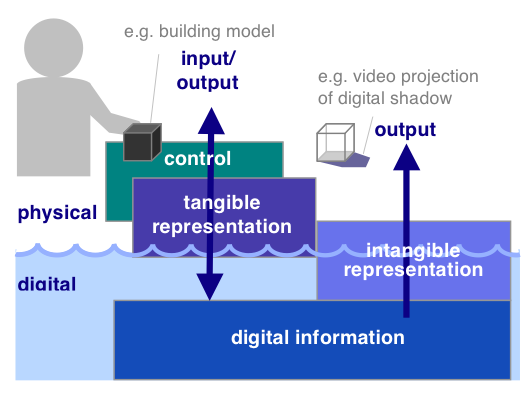
\includegraphics[height=3in]{img/ImplementierungUeberblick/MCRit.png}
	\caption[Überblick über das MCRit-Modell]{Überblick über das MCRit-Modell (entnommen aus \citet{Ishii08})}
	\label{fig:img_ImplementierungUeberblick_MCRit}
\end{figure}

Basierend auf der konzeptuellen Grundlage gibt \citeauthor{Ishii08} die grundlegenden Eigenschaften von \glspl{TUI} an:
\begin{description}
	\item[Computational Coupling] \emph{of tangible representations to underlying digital information and computation}. Der zentrale Aspekt jedes \gls{TUI} ist die Kopplung von realen Artefakten mit digitaler Information und diese Information manipulierende Funktionen. Zu berücksichtigen ist dabei die Art der Abbildung, also welche Prinzipien der Übersetzung und welche Metaphern (bei \citeauthor{Ishii08}: „Embodiment“) verwendet werden.
	\item[Embodiment of mechanisms for interactive control] \emph{with tangible representations}. In \glspl{TUI} werden die physischen Repräsentationen des Systemzustandes gleichzeitig auch zur Steuerung des Systems verwendet. Von Interesse sind hier die Fähigkeiten des Tangibles selbst (“inert“, also passive Objekt, die durch Benutzer manipuliert werden müssen oder „actuated“, also aktive Elemente, die selbständig Änderungen des Systemzustandes ausgeben können), die Beschränkung des Interaktionsraums (“unconstrainted“ -- unbeschränkt, „weakly constrainted“ -- nur schwach eingeschränkt, wie bei der Interaktion auf Oberflächen, oder „tightly constrainted“ -- stark eingeschränkt, z.B. bei Tokens, die nur entlang einer Achse bewegt werden können) sowie die durch die physische Form der Tokens und die Constraints vorgegebenen bzw. angedeuteten Interaktionen und deren Kohärenz mit der dadurch manipulierten digitalen Information.
	\item[Perceptual Coupling] \emph{of tangible representations to dynamic intangible representations}. Die wahrgenommene Koppelung zwischen dem physischen Anteil des Systemzustandes und dem intangiblen (z.B. projizierten oder akustischen) Anteil ist der dritte wichtige Aspekt, der beim Design von Tangible Interfaces zu berücksichtigen ist. Der kritische Faktor ist dabei nach \citeauthor{Ishii08} die Reaktion des intangiblen Anteil auf Änderung des tangiblen Anteils in Echtzeit. Zwischen der Manipulation von physischen Elementen und eine adäquaten Reaktion des Systems, die sich auch auf die intangible Repräsentation auswirkt, darf nur minimale, idealerweise nicht als solche wahrgenommene Verzögerung liegen. 
\end{description}

Je nach Ausprägung dieser Eigenschaften können sich \glspl{TUI} in unterschiedliche Kategorien von Systemen manifestieren. Basierend auf den bereits von \citet{Ullmer05} angegebenen Kategorien (siehe Abschnitt \ref{sub:tokens_und_constraints_nach_ullmer}) erweitert \citeauthor{Ishii08} das Schema und identifiziert acht Kategorien von \glspl{TUI}:
\begin{description}
	\item[Tangible Telepresence] Systeme, bei denen entfernte physische Objekte digital miteinander gekoppelt werden, so dass Manipulationen eines Objekts an den gekoppelten Objekten physisches Feedback auslösen können. Durch die Koppelung zwischen entfernter Ein- und Ausgabe können Präsenz-Aspekte auch in dissoziierten Anwendungsfällen übermittelt werden.
	\item[Tangibles with kinetic Memory] Systeme, die Manipulation physischer Objekte aufnehmen und diese Manipulationen auch wieder physisch wiedergeben können.
	\item[Constructive Assembly] Entspricht der von \citet{Ullmer05} angegebenen Kategorie und umfasst Systeme, bei denen der Systemzustand durch die (physische) Verknüpfung von physischen Elementen repräsentiert und manipuliert wird.
	\item[Tokens and Constraints] Entspricht der von \citet{Ullmer05} angegebenen Kategorie und umfasst Systeme, die informationstragende physische Elemente zur Repräsentation des Systemzustandes benutzen und die möglichen Interaktionen mittels ebenfalls physischer Constraints beschränken bzw. vorgeben.
	\item[Interactive Surfaces -- Tabletop UI] Entspricht der von \citet{Ullmer05} angegebenen Kategorie und umfasst Systeme, bei denen physische Objekte auf einer Oberfläche manipuliert werden, um den Systemzustand zu verändern. Dabei wird meist zusätzlich visuelles Feedback auf der Oberfläche ausgegeben, wodurch Eingabe- und Ausgabemedium kohärent sind.
	\item[Continuous Plastic TUI] Umfasst Systeme, die in der Lage sind, die äußere Form ihrer physischen Repräsentationen zu verändern bzw. auf derartige Formänderungen mit Änderungen des Systemzustandes reagieren.
	\item[Augmented Everyday Objects] Systeme, bei denen physische Objekte des Alltagslebens mit Technologie ausgestattet werden, die einen wie auch immer gearteten Mehrwert bei der Benutzung bieten kann.
	\item[Ambient Media] Systeme, bei denen interaktive Systeme durch Zusatzinformation ergänzt werden, die nicht von der eigentlichen Arbeitsaufgabe ablenken. Im engeren Sinne handelt es sich dabei nach \citeauthor{Ishii08} nicht um ein \gls{TUI}, die Kategorie hat aber insofern Relevanz, als dass nicht die herkömmlichen Ausgabekanäle (wie Bildschirme) benutzt werden um digitale Information zu repräsentieren.
\end{description}

Grundlegend gemein sind jedoch allen Arten von Systemen ein Satz von Merkmalen, die sie in ihrer Eigenschaft als \glspl{TUI} mitbringen und die sich dem Autor zufolge durchwegs vorteilhaft auf die Interaktion mit den Benutzern auswirken können:
\begin{description}
	\item[Double Interaction Loop -- Immediate Tactile Feedback] Tangible User Interfaces verfügen inhärent über zwei Feedbackschleifen, über die den Benutzern Reaktionen auf deren Eingaben rückgespiegelt werden. Die erste, unmittelbare, Feedback-Schleife ist die haptische Erfahrung bei der Manipulation der physischen Element. Die Reaktion ist sofort sichtbar und muss nicht durch das System erfasst, interpretiert und ausgegeben werden. Die zweite Schleife wird über die intangible Repräsentation des Systemzustands realisiert, auf der sich ebenfalls Reaktionen auf Benutzereingaben manifestieren. Dabei muss die Benutzerinteraktion jedoch erfasst und interpretiert werden, bevor eine adäquate Reaktion erstellt und ausgegeben werden kann. Diese Reaktion kann umfassender als in der ersten Schleife ausfallen, benötigt jedoch mehr Zeit.
	\item[Persistency of Tangibles] Bei \glspl{TUI} wird ein wesentlicher Anteil des Systemzustandes durch die Konfiguration des physischen Elemente dargestellt. Diese sind ihrer Natur nach persistent, repräsentieren diesen Anteil des Systemzustandes also unabhängig von etwaiger Infrastruktur und sind auch verfügbar, wenn diese abgeschaltet ist.
	\item[Coincidence of Input and Output Spaces] Ein grundlegendes Designkriterium von \glspl{TUI} ist die Kohärenz (bei \citeauthor{Ishii08}: Koinzidenz) von Eingabe- und Ausgabekanälen. Dies ermöglicht eine nahtlose Interaktion und Informationsrepräsentation im physischen und digitalen Raum. 
	\item[Special Purpose vs. General Purpose] In Abgrenzung zu \glspl{GUI}, die im Normalfall zur Interaktion mit beliebigen Applikationen verwendet werden können, sind \glspl{TUI} eher spezifisch auf einen bestimmten Anwendungsfall hin ausgerichtet und und werden dementsprechend konzipiert. Wichtig ist hier vor allem die Berücksichtigung den Benutzern vertrauter Metaphern bei der Konzeption der Informationsrepräsentation und der Manipulations-Werkzeuge.
	\item[Space-Multiplexed Input] Generell ermöglichen \glspl{TUI} eine parallele Manipulation mehrerer räumlich verteilter physischer Objekte zur gleichen Zeit. Es ist damit möglich kollaborative Interaktion zu unterstützen, bei der mehrere Benutzer den Systemzustand simultan beeinflussen. Die Kollaboration kann dabei auch räumlich verteilt stattfinden, wenn Mechanismen existieren, die den Systemzustand der einzelnen \gls{TUI}-Instanzen synchron hält (z.B. durch Aktuatoren). 
\end{description}

Im seinen Schlussbetrachtungen führt \citeauthor{Ishii08} die größten Mängel des noch jungen Forschungsgebiets der Tangible User Interfaces aus: es fehle an „Killer Applications“, an skalierbaren Toolkits und an verlässlichen und validierten Design Prinzipien.
\\[1em]
\begin{tabular}{| p{3cm} | p{10cm} |}
  \hline
  Kategorien & Tangible Telepresence, Tangibles with kinetic Memory, Constructive Assembly, Tokens and Constraints, Interactive Surfaces -- Tabletop UI, Continuous Plastic TUI, Augmented Everyday Objects, Ambient Media \\ \hline
  Konzepte & Digital Information, Tangible Representation, Control, Intangible Representation \\ \hline
  Eigenschaften & \emph{Gesamtsystem}: Computational Coupling, Embodiment of Control Mechanisms, Perceptual Coupling \\ \hline
  PD-Brücke & Abhängig von der Art des Systems, grundsätzlich aber immer Koppelung zwischen tangibler Repräsentation und Control \\ \hline
\end{tabular} 

% subsection tangible_bits_beyond_pixels (end)

\subsection{Zusammenfassung} % (fold)
\label{sub:tui_konzepte_zusammenfassung}

Die in den vorhergehenden Abschnitten betrachteten Arbeiten sind in Ansatz, Ausgangspunkt und Vorgehensweise höchst unterschiedlich. Ihnen ist jedoch gemein, dass sie sich mit der Konzeptualisierung von Tangible User Interfaces beschäftigen. Die Arbeiten können dabei entlang zweier Dimensionen nach Ziel und Betrachtungsgegenstand klassifiziert werden. Hinsichtlich der Zielsetzung sind Arbeiten, die auf die Spezifikation eines \gls{TUI} ausgerichtet sind, von solchen zu unterscheiden, die auf die Evaluation existierender Systeme ausgelegt wurden (im Sinne von detailliert angegebenen Merkmalen, die ein System aufweisen muss um eine bestimmte Eigenschaft zu haben). Als dritte Ausprägung sind noch Ansätze zu identifizieren, die eine Einordnung in einen Referenzrahmen ermöglich sollen, ohne die Eigenschaften des \gls{TUI} im Detail zu betrachten. Hinsichtlich des Betrachtungsgegenstandes sind unterschiedliche Detaillierungsgrade zu erkennen, wobei hier die beiden Ausprägungen „Gesamtsystem“ und „einzelne physische Elemente“ als Extremwerte zur Klassifikation herangezogen werden. Hinsichtlich des Betrachtungsgegenstandes ist noch zu unterscheiden, ob sich die Arbeit auf die Struktur des \gls{TUI} konzentriert oder sich darüber hinaus auch explizit mit dessen Verwendung beschäftigt. Ansätze der zweiten Art werden in der Tabelle kursiv gesetzt. Jeder Ansatz verfolgt über diese Einordnung hinaus noch spezifische Zielsetzungen, die der Übersichtlichkeit wegen in dieser ersten Einordnung nicht angegeben werden. 

Die Einordnung in die Kategorien (siehe Tabelle \ref{tab:tui_konzeptkategorien}) erfolgt aufgrund der von den jeweiligen Autoren in den Artikeln explizit genannten Zielsetzungen oder -- wenn diese nicht vorhanden oder aussagekräftig sind -- aufgrund der von Autoren gewählten Schwerpunktsetzungen und unter Berücksichtigung des jeweiligen Gesamtzusammenhangs (übergeordnetes Forschungsvorhaben). Ansätze, die zu mehreren Kategorien Beiträge liefern, werden in allen betreffenden Feldern angeführt.

\begin{table}[htbp]
	\centering
	\caption[Kategorien von konzeptuellen Arbeiten im Gebiet Tangible User Interfaces]{Kategorien von konzeptuellen Arbeiten im Gebiet Tangible User Interfaces (kursiv gesetzte Arbeiten gehen auch auf das Verhalten von TUIs ein)}
	\begin{tabular}{| p{2,5cm} || p{5,5cm} | p{5,5cm} |} \hline
		 & Gesamtsystem & einzelne physische Elemente \\ \hline \hline
		Spezifikation & Bricks\linebreak MCRpd-Interaktions-Modell\linebreak Tangible Bits: Beyond Pixels & Containers, Tokens und Tools\linebreak Tokens+\-Constraints\linebreak \emph{Tokens and Constraints nach Shaer et al.}\\ \hline
		Evaluation & Graspable User Interfaces & \emph{Taxonomie für Tangible User Interfaces} \\ \hline
		Einordnung & Tangible Bits\linebreak Tokens+\-Constraints\linebreak Kategorien von TUI Anwendungen\linebreak Tangible Bits: Beyond Pixels & Tangible Objects Meaning\linebreak Degree of Coherence \\ \hline
	\end{tabular}
	\label{tab:tui_konzeptkategorien}
\end{table}

In dieser Aufstellung ist zu erkennen, dass ein Großteil der Ansätze nicht auf den Interaktionsaspekt des Anwendungsfalls eingeht, für den das betrachtete \gls{TUI} konzipiert ist, sondern sich auf die strukturellen Aspekte des Systems beschränkt.  

Den umfassendsten Ansatz zur Spezifikation bietet die Arbeit „Tokens and Constraints“ von \citep{Shaer04}, der aufbauend auf der Arbeit von \citet{Ullmer02} einen modifizierten Token+Constraints-Ansatz vorstellt. Dieser eignet sich durch ein breiteres Verständnis des Constraint-Begriffs für die allgemeine Spezifikation der Struktur eines TUI. Zusätzlich stellt er ein Schema zur Verfügung, in dem -- basierend auf der Struktur -- auch das Verhalten des Systems spezifiziert werden kann.

Zur detaillierten Evaluation eines \gls{TUI} bietet sich die Taxonomie von \citet{Fishkin04} an, der in seiner Arbeit in zwei Dimensionen sowohl die Betrachtung der Struktur als auch der Verwendung der Objekte eines \gls{TUI} in den spezifizierten Interaktionsabläufen erlaubt.

\subsubsection{Ausdrucksstärke der konzeptuellen Ansätze} % (fold)
\label{ssub:ausdrucksstärke_der_konzeptuellen_ansätze}

Grundsätzlich sind jene Ansätze, die sich mit der detaillierten Beschreibung eines \gls{TUI} befassen, ausdrucksstärker als jene Ansätze, die ein System lediglich global betrachten. Dies bezieht sich jedoch in erster Linie auf die Quantität der generierten Daten, qualitativ gesehen ergänzen beide Sichtweisen einander und sind sowohl bei Spezifikation als auch Evaluation komplementär anzuwenden. Der Fokus der Betrachtung der jeweiligen Ansätze ist in Tabelle \ref{tab:tui_konzeptkategorien} angeführt und wird hier nicht separat unterschieden.

Einige der vorgestellten Ansätze sind inhaltlich insofern als überholt anzusehen, als dass sie heute gängige Techniken und Interaktionsparadigmen nicht adäquat abbilden können. Dies gilt sowohl in struktureller Hinsicht als auch in Bezug auf das Verhalten eines Systems. Die strukturellen Konzepte haben sich konzeptuell von „werkzeug-zentrierten“ auf „informations-zentrierte“ Sichtweise weiter entwickelt. Ältere, „werkzeug-zentrierte“ Ansätze betrachten die physischen Elemente ausschließlich als Werkzeuge zur Manipulation digitaler Information, die nach wie vor herkömmlich visuell ausgegeben wird und keine physische Manifestation besitzt. Typische Vertreter dieser Sichtweise sind die Arbeiten von \citet{Fitzmaurice95} und \citet{Fitzmaurice96}. Ab der Arbeit von \citet{Ishii97} wird der Aspekt der physischen Repräsentation von Information berücksichtigt, womit erstmals eine umfassende Beschreibung von Systemen ermöglicht wird, die heute als \gls{TUI} bezeichnet werden.

In der Folge wurden unterschiedliche Ansätze vorgestellt, die auf verschiede Aspekte in der Beschreibung der Struktur eingehen. Ein grundlegendes Unterscheidungsmerkmal der Ansätze ist ihre Herangehensweise an die Unterscheidung zwischen physischen Objekten, die Information repräsentieren und solchen, die Information manipulieren (in wenigen Fällen werden auch Werkzeuge zur Systemsteuerung separat betrachtet). Eine Herangehensweise ist die strikte konzeptuelle Trennung zwischen physischen Objekten, die zur Informationsrepräsentation verwendet werden und solchen, die als Werkzeug zur Manipulation eingesetzt werden. Typische Vertreter sind hier die Arbeiten von \citet{Ishii97} und \citet{Holmquist99}. Dem hingegen steht die Herangehensweise die Bedeutung eines physischen Objekts für eine bestimmte Anwendung auf einem Kontinuum einzuordnen und Objekte damit als eher „werkzeug-artig“ oder eher „repräsentations-artig“ (oder beides integrierend) einzuordnen. Typische Vertreter für diese Herangehensweise sind die Arbeiten von \citet{Underkoffler99}, \citet{Koleva03} und \citet{Fishkin04}. Einen dritten Weg gehen die Ansätze von \citet{Ullmer00} und darauf aufbauend \citet{Ishii08}, die physische Elemente immer als Kombination eines Repräsentations- und Kontroll-Anteils sehen und diese konzeptuell separat behandeln. Implizit in dieser Tradition stehen auch die Ansätze von \citet{Ullmer02} und \citet{Shaer04}, die mit dem „Tokens und Constraints“-Konzept einerseits eine dritte Art von physischen Objekten -- die Constraints, die den Interaktionsraum beschränken -- einführen, andererseits aber bei den eigentlich zur Interaktion verwendeten physischen Elementen nicht zwischen Repräsentationen und Werkzeugen unterscheiden. Funktionalität wird vielmehr durch die Manipulation eines (informationstragenden) Tokens im Kontext von Constraints ausgelöst -- Tokens haben somit einen Kontroll-Aspekt im Sinne von \citet{Ullmer00}.

Seltener anzutreffen sind Arbeiten, die explizit auf die Beschreibung oder Evaluation der Interaktionsabläufe eines \gls{TUI} eingehen. \citet{Fishkin04} behandelt diesen Aspekt im Rahmen der „Metaphor“-Dimension seiner Taxonomie. Er unterscheidet dort zwischen \glspl{TUI} oder \gls{TUI}-Komponenten, deren Interaktionsmetaphern eher an Objekten der realen Welt und / oder an Tätigkeiten der realen Welt angelehnt sind. Werden alle Komponenten eines \gls{TUI} in diese Dimension eingeordnet, so ermöglicht dies die Prüfung, ob die Metaphern konsistent gewählt wurden  
\citep{Oppl09d}. Die Interaktionsabläufe im Detail sind jedoch bei \citet{Fishkin04} nicht Gegenstand der Betrachtung. Auf detaillierter Ebene gehen lediglich \citet{Shaer04} auf Interaktionsabläufe im Allgemeinen und der Spezifikation im Speziellen ein. Die Autoren erweitern dazu den Token+Constraints-Ansatzes \citep{Ullmer02} um einen Interaktionsaspekt, der auf Basis der strukturellen Eigenschaften eines \gls{TUI} deren dynamisches Zusammenspiel untereinander und mit den Benutzern festlegt. Damit wird es möglich, ein \gls{TUI} sowohl in Struktur als auch Verhalten umfassend zu spezifizieren.
% subsubsection ausdrucksstärke_der_konzeptuellen_ansätze (end)

\subsubsection{Nomenklatur}

Hinsichtlich der Bezeichnung der Elemente eines \gls{TUI} existiert keine einheitliche Nomenklatur, die konsistent über mehrere Arbeiten hinweg verwendet wird. Die Tabellen \ref{tab:tui_nomenklatur1} und \ref{tab:tui_nomenklatur2} gibt eine Übersicht über die für die einzelnen konzeptuellen Elemente verwendeten Begriffe.

\begin{table}[htbp]
		\centering
	\caption{Gegenüberstellung der Nomenklatur zur Beschreibung der Elemente eines TUI -- Teil 1}  
	\begin{tabular}{|p{2.2cm}||p{3cm}|p{3cm}|p{2cm}|p{2cm}|} \hline
			Arbeit & physisches Objekt zur Informations\-repräsentation & physisches Werkzeug zur Informations\-manipulation & physische Beschränkung des Interaktionsraums & digitale Objekte \\ \hline \hline
		
		Bricks & --- & Brick & --- & --- \\ \hline
		Graspable User Interfaces & --- & --- & --- & --- \\ \hline
		Tangible Bits & Phicon & Phandle (Informationsmanipulation), Instrument (Systemsteuerung) & Tray & --- \\ \hline
		Containers, Tokens und Tools & Container (unspezifische Form), Token (spezifische Form) & Tool & --- & --- \\ \hline
		Tangible Objects Meaning & Object as pure object (unspezifische Form), Object as attribute (teilspezifisch), Object as noun (spezifische Form) & Object as verb (fix gebundene Funktionalität), Object as reconfigurable tool (konfigurierbare Funktionalität) & --- & --- \\ \hline
		MCRpd Inter\-aktions-Modell &  Rep-P & Control & --- & Model, Rep-D (Manifestation)\\ \hline
	\end{tabular}

			\label{tab:tui_nomenklatur1}
\end{table}

\begin{table}[htbp]
		\centering
	\caption{Gegenüberstellung der Nomenklatur zur Beschreibung der Elemente eines TUI -- Teil 2}  
	\begin{tabular}{|p{2.2cm}||p{3cm}|p{3cm}|p{2cm}|p{2cm}|} \hline
			Arbeit & physisches Objekt zur Informations\-repräsentation & physisches Werkzeug zur Informations\-manipulation & physische Beschränkung des Interaktionsraums & digitale Objekte \\ \hline \hline
		Tokens + Constraints & Tokens & Tokens + Constraints & Constraints & --- \\ \hline
		Degree of Coherence & Identifier (unspezifische Form), Proxy (von hier an: spezifische Form, Enge der Bindung ansteigend), Projection, Illusion of same objects & General purpose tools (konfigurierbare Funktionalität), Specialized tools (fix gebundene Funktionalität) & --- & --- \\ \hline
		TAC & Token-Pyfo & Token-Pyfo & Constraint-Pyfo & Variable \\ \hline
		TUI-Anwendungs-Kategorien & --- & --- & --- & --- \\ \hline
		Taxonomie für TUIs & --- & --- & --- & --- \\ \hline
		Tangible Bits: Beyond Pixels & tangible Represen\-tation & Control & --- & digital information, intangible representation (Manifestation) \\ \hline
	\end{tabular}
	\label{tab:tui_nomenklatur2}
\end{table}


% \newcolumntype{C}[1]{>{\centering\arraybackslash}m{#1}}
% % \begin{center}
% \begin{longtable}{@{}p{0.04\textwidth}@{}p{0.72\textwidth}>{\RaggedLeft}p{0.12\textwidth}>{\RaggedLeft}p{0.12\textwidth}@{}}%
% \begin{longtable}{|p{2cm}||p{2cm}|p{2cm}|p{2cm}|p{2cm}|p{2cm}|} \hline
%  \caption{Gegenüberstellung der Nomenklatur zur Beschreibung der Elemente eines TUI}  \label{tab:tui_nomenklatur} \\
% 
% 	% 	Arbeit & 
% 	% 	physisches Objekt & 
% 	% 	physisches Objekt zur Informations\-repräsentation & 
% 	% 	physisches Werkzeug zur Informations\-manipulation & 
% 	% 	physische Beschränkung des Interaktionsraums & 
% 	% 	digitale Objekte \\ \hline \hline 
% 	% \endfirsthead
% 	
% 	%   \multicolumn{6}{c}{{\tablename} \thetable{} -- Fortsetzung} \\
% 	% \hline \\
% 	% 	Arbeit & physisches Objekt & physisches Objekt zur Informations\-repräsentation & physisches Werkzeug zur Informations\-manipulation & physische Beschränkung des Interaktionsraums & digitale Objekte \\ \hline \hline
% 	% \endhead
% 	% 
% 	%   \multicolumn{6}{r}{Fortsetzung auf der nächsten Seite\ldots} \\
% 	% \endfoot
% 	% 
% 	% %This is the footer for the last page of the table...
% 	%   \\ \hline
% 	% \endlastfoot
% 	
% 	Bricks & --- & --- & Brick & --- & --- \\ 
% 	Graspable User Interfaces & --- & --- & --- & --- & --- \\ 
% 	Tangible Bits & --- & Phicon & Phandle (Informationsmanipulation), Instrument (Systemsteuerung) & Tray & --- \\ 
% 	Containers, Tokens und Tools & --- & Container (unspezifische Form), Token (spezifische Form) & Tool & --- & --- \\ 
% 	Tangible Objects Meaning & Object & Object as pure object (unspezifische Form), Object as attribute (teilspezifisch), Object as noun (spezifische Form) & Object as verb (fix gebundene Funktionalität), Object as reconfigurable tool (konfigurierbare Funktionalität) & --- & --- \\
% 	MCRpd Inter\-aktions-Modell & Represen\-tation & Rep-P & Control & --- & Model, Rep-D (Manifestation)\\
% 	Tokens+\-Constraints & --- & Tokens & Tokens+\-Constraints & Constraints & --- \\
% 	Degree of Coherence & --- & Identifier (unspezifische Form), Proxy (von hier an: spezifische Form, Enge der Bindung ansteigend), Projection, Illusion of same objects & General purpose tools (konfigurierbare Funktionalität), Specialized tools (fix gebundene Funktionalität) & --- & --- \\ 
% 	TAC & Pyfo & Token & Token & Constraint & Variable \\ 
% 	Kategorien von TUI-Anwendungen & --- & --- & --- & --- & --- \\
% 	Taxonomie für TUIs & --- & --- & --- & --- & --- \\ 
% 	Tangible Bits: Beyond Pixels & Represen\-tation & tangible Represen\-tation & Control & --- & digital information, intangible representation (Manifestation)
% 	
% \end{longtable}
% % \end{center}

Diese Arbeit folgt in der Bezeichnung der physischen Elemente dem TAC-Ansatz von \citep{Shaer04} und verwendet generell der Begriff des \emph{„Tokens“}. Zur Abgrenzung wird, wo nötig, von „Modellierungstokens“ (jene Tokens, die Information repräsentieren) und „Werkzeugtokens“ (jene Tokens, die Funktionalität auslösen) unterschieden. Der digitale Aspekt eines \gls{TUI} wird selten explizit benannt, der von \citep{Shaer04} gewählte Begriff der „Variable“ erscheint im Kontext der Repräsentation von Modellen aber als zu spezifisch bzw. unpassend vorbelegt. Deshalb wird im Allgemeinen nach \citep{Ishii08} von \emph{„digitaler Information“} gesprochen, wenn explizit auf die digitale Repräsentation des Modells Bezug genommen wird, wird der Begriff \emph{„Modell-Elemente“} verwendet. Eine weitere Ausdifferenzierung der Nomenklatur zur Bezeichnung von anwendungsspezifischen Eigenschaften des hier vorgestellten Werkzeugs erfolgt im Rahmen der folgenden Kapitel.

Die hier vorgestellten Ansätze werden nach der Beschreibung des Werkzeugs in Kapitel \ref{cha:konzeptuelle_evaluierung} wieder aufgegriffen und auf das hier entwickelte System angewandt. Damit werden zwei Ziele verfolgt. Einerseits soll die praktische Anwendbarkeit der Ansätze und deren Verwendbarkeit für ein konkretes, im Vergleich zu den in den Artikeln vorgestellten Beispielen komplexes und flexibles System überprüft werden. Andererseits soll versucht werden, aus der theoretisch-konzeptuellen Betrachtung des Werkzeugs Inkonsistenzen im Design zu erkennen und potentiell verbesserungswürdige Aspekte des Werkzeugs zu identifizieren. Eine Gegenüberstellung mit den Ergebnissen der praktischen Evaluierung erlaubt in der Folge auch die Überprüfung des Aussagekraft derartiger auf theoretischen Konzepten basierenden Betrachtungen bzw. Spezifikationen.

% subsection tui_konzepte_zusammenfassung (end)

% section konzeptualisierungen_von_tangible_interfaces (end)

\section{Tabletop Interfaces} % (fold)
\label{sec:tabletop_interfaces}

Tabletop Interfaces sind Benutzungsschnittstellen, bei denen die Interaktion mit einem Computersystem über eine (im Allgemeinen horizontal angebrachte) Tischplatte durchgeführt wird. Tabletop Interfaces sind nicht als echte Untermenge von Tangible Interfaces zu sehen. Systeme, bei denen die Interaktion mittels direkter Berührung der Oberfläche mit den Händen („Touch-“ bzw. „Multitouch“-Systeme) durchgeführt wird, werden ebenfalls zu den Tabletop Interfaces gezählt, sind aber aufgrund des fehlenden physischen Repräsentationsaspekts des Systemzustandes nicht als unbedingt als Tangible Interface zu klassifizieren.

Im Sinne einer Aufarbeitung der „Related Work“ beschränkt sich diese Arbeit hier auf jene Systeme, die historisch für die Entwicklung des Feldes der „Tangible Tabletop Interfaces“ wichtig waren bzw. sind und jene Arbeiten, in denen inhaltlich ähnliche Zielsetzungen wie in dieser Arbeit verfolgt wurden, auch wenn das zugrunde liegende Tabletop Interface keine „tangiblen“ Aspekte aufweist.

\subsection{Historische Entwicklung} % (fold)
\label{sub:historische_entwicklung_von_tabletop_interfaces}

Tabletop Interfaces wurden erstmals von \citet{Wellner93a} beschrieben, der damit gemäß der Vision „back to the real world“ \citet{Wellner93} beabsichtigte, die Trennung zwischen der realen Welt und dem digitalen Inforamtionsraum zu beseitigen und eine nahtlose, natürliche Interatkion mit Computersystemen zu ermöglichen. Im Bereich der Tangible Interfaces wurde bereits mit der Einführung des Begriffs von \citet{Ishii97} die Geräteklasse der „Interactive Surfaces“ identifiziert, in die Systeme eingeordnet wurden, die eine mit digitaler Information angereicherte physische Oberfläche als Ausgabemedium verwenden, auf der zur Eingabe physische Objekt manipuliert werden. Diese Klasse von Systemen ist nicht auf Tische eingeschränkt, sondern umfasst z.B. auch digital augmentierte Wände. Das MetaDESK-System, das in der gleichen Arbeit als Beispiel für Interactive Surfaces vorgestellt wird, kann als das erste in der Literatur beschriebene Tangible Tabletop Interface bezeichnet werden. 

Frühere Arbeiten, wie die von \citet{Fitzmaurice96} beschriebenen „Bricks“, setzten zur Interaktion physische Bausteine ein, die lediglich einen Bezug zueinander aufweisen, aber keine gemeinsame Oberfläche als Referenzrahmen benötigen und verwenden ("relational interfaces" im Sinne von \citet{Ullmer00}). Fasst man den Begriff der Interactive Surfaces nach \citet{Ishii97} eng, so fallen derartige Systeme aufgrund des fehlenden gemeinsamen physischen Referenzrahmens nicht in diese Klasse. In jenen Fällen, in denen trotzdem ein räumlich entsprechend begrenztes physisches „Trägermedium“ benötigt wird (also eine klassische, nicht digital augmentierte Tischoberfläche zur Anordnung der Elemente des Interfaces eingesetzt wird), kann trotzdem von einem „Tangible Tabletop Interface“ gesprochen werden.

\subsubsection{Anfänge} % (fold)
\label{subs:anfaenge}

Das Sensetable-System \citep{Patten01} ist die erste in der Literatur beschriebene „Interactive Surface“ Plattform, die breit in unterschiedlichen Anwendungsszenarien eingesetzt wurde. Es steht inhaltlich in der Tradition des MetaDESK-Systems \citep{Ishii97} und basiert technologisch auf eine Tischoberfläche, auf die von oben projiziert wird und mit der mittels auf die Oberfläche aufgesetzten „Pucks“ interagiert werden kann. Die Feststellung der Position der „Pucks“ erfolgt mittels einem magnetischem Positionierungssystem. Die Positionsbestimmung auch mehrerer Objekte gleichzeitig kann damit quasi verzögerungsfrei und mit einer Genauigkeit im mm-Bereich durchgeführt werden.

Das BUILD-IT-System \citep{Fjeld01} ist eines der ersten Systeme, in dem Tabletop Interfaces zur Unterstützung von kooperativen Arbeitsprozessen eingesetzt werden. \citet{Fjeld97} führen den Begriff des „Natural User Interfaces“ und meinen damit die kohärente Manipulierbarkeit von Objekten auf physischen und digitalen Oberflächen. In der konkreten Implementierung des BUILD-IT-Systems \citep{Fjeld01} steht eine horizontale Oberfläche zur Verfügung, auf der physische Objekte platziert werden können und auf die synchron anwendungsspezifische Information projiziert wird. Zusätzlich steht eine vertikale Oberfläche zur Erweiterung der Darstellungsraums zur Verfügung, auf der lediglich Information angezeigt wird, während eine physische Manipulation nicht möglich ist. Das System wurde in unterschiedlichen Anwendungsszenarien zum Einsatz gebracht, und einer Evaluierung hinsichtlich seiner Benutzbarkeit und seinen Auswirkungen auf die Arbeit der Benutzer unterzogen. Die Ergebnisse dieser Untersuchung sprechen im Wesentlichen für die Nützlichkeit von Tabletop User Interfaces, auch wenn aufgrund technischer Restriktionen die Verwendbarkeit des Systems eingeschränkt war. Die Wirkung des Systems auf kooperative Arbeit wurde explizit nicht untersucht.  

% subsection historische_entwicklung_von_tabletop_interfaces (end)

\subsection{Aktuelle Plattformen} % (fold)
\label{sub:aktuelle_plattformen}
Mit dem stärker werdenden Forschungsinteresse im Bereich der Tabletop Interfaces und dem zunehmenden kommerziellen Interesse ist in den letzten Jahren die zunehmende Verfügbarkeit von Applikationsplattformen für Tabletop Interfaces zu beobachten, die sowohl einen definierten Satz von Hardware-Funktionalität (also dem eigentlichen Tabletop Interface) als auch eine Programmierschnittstelle für die Entwicklung eigener Applikationen mit sich bringt. Mit Stand von Ende 2009 werden in der aktuellen Forschung vor allem drei Lösungen eingesetzt, von denen zwei auch die Hardware kommerziell vertreiben und eine lediglich die Software und Bauanleitungen für das Tabletop Interface anbietet. Absehbar ist hier die weitere Diversifizierung des Angebots, wobei auf die neueren Anbieter an dieser Stelle jedoch nicht weiter eingegangen wird.

\subsubsection{ReacTable} % (fold)
\label{ssub:reactable}

Der ReacTable \citep{Kaltenbrunner06} ist ein auf einem Tangible Tabletop Interface beruhendes kooperatives Musikinstrument, dessen Hardwarekomponente und Software-Schnittstelle zur visuellen Identifikation von Objekten auf der Oberfläche generisch einsetzbar sind. Die Hardware des ReacTable besteht aus einem Tisch, dessen Oberfläche semitransparent ausgeführt ist. Die Objekte werden durch auf deren Unterseite angebrachten visuellen Markern identifiziert. Zugleich wird von der Unterseite mittels einem Projektor zusätzliche Information auf die Oberfläche projiziert.

Die zur Objektidentifikation verwendeten Marker sind proprietär und bilden einen eindeutigen Code ab, der softwareseitig das ensprechende Element identifiziert. Die Anzahl der Marker ist erweiterbar, wobei deren Form frei gewählt werden kann. Zusätzlich zu Identifikation von Elementen kann die Software auch Fingerberührungen visuell erkennen, wodurch die Oberfläche multi-touch-fähig wird.

Die Software ist plattformübergreifend für Windows, Mac OS X und Linux als Open Source Software verfügbar. Die Analyse des Kamerabilds erfolgt in Quasi-Echtzeit mit 15 bis 20 Bildern pro Sekunde (abhängig vom eingesetzten Rechner). Die Information für auf der Oberfläche erkannte Elemente oder Finger wird über das proprietäre aber mittlerweile auch von anderen Anbietern eingesetzte TUIO-Protokoll über einen \gls{UDP}-Port ausgegeben und kann so von beliebigen Clients übernommen und verarbeitet werden. In den Softwarepaketen sind vorgefertigte Clients für die Programmiersprachen C und Java enthalten.

% subsubsection reactable (end)

\subsubsection{Microsoft Surface} % (fold)
\label{ssub:microsoft_surface}

Die Microsoft Surface\footnote{http://www.microsoft.com/surface/} ist ein kommerzielles Produkt, dass als Paket von Hard- und Software von Microsoft vertrieben wird. Die Hardwarekomponente stellt sich als ein in sich abgeschlossenes System ohne vorgesehene Manipulationsmöglichkeit der Benutzer oder Entwickler dar. Sie besteht dabei aus einer Tischoberfläche, die semitransparent ausgeführt ist und von unten projiziert wird. Die Erfassung von Benutzerinteraktion erfolgt visuell mittels unter der Oberfläche installierten Kameras. Der Fokus liegt dabei auf der Identifikation von Berührungen mit einem oder mehreren Fingern bzw. durch eine oder mehrere Personen. Zusätzlich können Objekte durch ihren Umriss oder durch proprietäre visuelle Codes identifiziert werden. Die Identifikation erfolgt dabei in Quasi-Echtzeit mit mehreren Bildern pro Sekunde (exakte Werte unbekannt). Der Tisch selbst ist in Form und Bauhöhe eher als Besprechungs- bzw. Bartisch denn als Arbeitstisch ausgeführt.

Softwareseitig kommt ein modifizierte bzw. erweitere Version von Windows Vista zum Einsatz. Die Microsoft Surface bietet neben einer Reihe von vorinstallierten Anwendungen auch die Möglichkeit, mittels einem \gls{API} auf die Information der Oberfläche identifizierten Objekte und Finger zuzugreifen und diese in eigenen Anwendungen zu verarbeiten. Diese Anwendungen müssen auf Microsoft's .NET-Framework basieren, um an das \gls{API} angebunden werden zu können. 

% subsubsection microsoft_surface (end)

\subsubsection{DiamondTouch} % (fold)
\label{ssub:diamond_touch}

Der DiamondTouch \citep{Dietz01} ist ein Projekt von den Mitsubishi Research Labs\footnote{http://www.merl.com/projects/DiamondTouch/}, dass mittlerweile kommerziell von dem Unternehmen Circle Twelve\footnote{http://www.circletwelve.com/} vertrieben wird. Im Gegensatz zu den anderen beiden vorgestellten Ansätzen setzt der DiamondTouch kein visuelles Identifikationverfahren ein, sondern verwendet ein auf kapazitiver Erkennung basierendes Verfahren, dass durch seine Ausführung nicht nur die Identifikation mehrerer gleichzeitiger Berührungen sondern auch die eindeutige Identifikation von Benutzern (auch über die Zeit bei nicht ununterbrochener Berührung) ermöglicht. Das System unterstützt jedoch keine Identifkation von Objekten, es können lediglich Berührungen identifiziert werden. Die Hardwareausführung ähnelt jener der Microsoft Surface, allerdings wird im Gegensatz zu den anderen beiden Lösungen von oben auf die Oberfläche projiziert. Um eine eindeutige Identifikation der handelnden Personen gewährleisten zu können, müssen diese außerdem auf je einem von bis zu vier an dem System angeschlossenen Stühlen sitzen.

Die Identifikations-Software arbeitet unter Windows oder Linux und liefert über ein \gls{API} die Berührungsinformation an eine vom Entwickler zu erstellende Applikation. Das \gls{API} kann dabei aus unterschiedlichen gängigen Programmiersprachen (wie C++, Java oder Adobe Flash) angesprochen werden.

% subsubsection diamond_touch (end)
% subsection aktuelle_plattformen (end)
% section tabletop_interface (end)

\section{Tabletop Interfaces zur Erstellung diagrammatischer Modelle} % (fold)
\label{sub:tangible_interfaces_zur_modellbildung}

In diesem Abschnitt werden Systeme beschrieben, die sich der Erstellung diagrammatischer Modelle auf tischbasierten Benutzungsschnittstellen widmen, also ein zu dieser Arbeit verwandtes Werkzeug mit verwandter Technologie umsetzen. Die eigentliche Zielsetzung unterscheidet sich im Einzelfall, die Verwandtschaft beschränkt sich auf die Unterstützung im Vorgang der Modellbildung.

Nicht betrachtet werden hier Systeme, die sich zwar mit Modellbindung im weiteren Sinne beschäftigen, deren Betrachtungsgegenstand aber nicht diagrammatische Modelle sind. Derartige Systeme haben oft den Anspruch, die Modellbildung weniger abstrakt zu gestalten und vor allem die Modellverwendung durch Simulationen an das Verhalten des dargestellten Phänomens in der realen Welt anzunähern. Ein klassisches Beispiel ist hier Urp \citep{Underkoffler99}, ein Stadtplanungssystem, bei dem Objekte, die Gebäude repräsentieren, maßstabsgetreu auf einer Oberfläche platziert werden können. Je nach ausgeführter Simulation können in Echtzeit die Lichtverhältnisse bei Sonneneinstrahlung oder die Luftströmungen im arrangierten Gebäude-Ensemble verfolgt werden. Systeme dieser Klasse beschäftigen mit anderen Aspekten von Modellbildung und vernachlässigen explizite Repräsentation der konzeptuellen Beziehungen zwischen Modellelementen. Sie sind deshalb nicht als verwandte Arbeiten zu klassifizieren.

Im ersten Unterabschnitt werden Systeme betrachtet, die sich historisch mit der Thematik der Modellierung mittels Tangible (Tabletop) Interfaces beschäftigen. Der zweiter Unterabschnitt stellt zwei Arbeiten vor, die parallel zur vorliegenden Arbeit entwickelt wurden und sich so wie diese mit den konkreten Modellierungsaufgaben im Rahmen von Concept Mapping beschäftigen, das, wie in Kapitel \ref{cha:methodik} beschrieben, auch eine methodische Grundlage dieser Arbeit darstellt. 

\subsection{Historische Entwicklung} % (fold)
\label{sub:historische_entwicklung}

Die Unterstützung der Bildung von diagrammatischen Modellen mittels Tangible Interfaces wird seit der Jahrtausendwende in der Literatur behandelt. Tatsächlich sind jedoch nur drei Arbeiten zu identifizieren, die sich mit der Bildung diagrammatischer Modelle beschäftigen und in der Literatur so ausführlich beschrieben sind, dass eine Berücksichtigung an dieser Stelle möglich ist. Zu diesen Arbeiten existieren jeweils mehrere Publikationen, als Referenz wurde hier jeweils jene Publikation herangezogen, in der das System am ausführlichsten dokumentiert ist.

\subsubsection{Tangible Business Process Analyser} % (fold)
\label{ssub:tangible_business_process_analyser}

Historisch wurde der Anwendungsfall der Modellbildung mit Tangible Interfaces bereits auf der ersten funktionsfähigen „Interactive Surface“, dem Sensetable \citep{Patten01}, umgesetzt. Der „Tangible Business Process Analyser“ \citep{Mori04} ist eine Anwendung, die auf Basis des Sensetable implementiert wurde und dazu dient, Workflows zu modellieren, deren Parameter einzustellen und in der Folge die Ergebnisse einer Simulation zu visualisieren. Das Modell selbst hat dabei keine physische Ausprägung sondern wird lediglich projiziert. Wie in vielen Systemen aus dieser Generation von Tangible Tabletop Interfaces (z.B. auch \citep{Fitzmaurice95}) werden auch in dieser Arbeit nur die Manipulations-Werkzeuge selbst physisch ausgeführt. Die Repräsentation der Information (hier: das Modell) verbleibt digital und wird z.B. durch Projektion auf die Tischoberfläche dargestellt. Die Manipulation der Modellelemente selbst sowie der zur Simulation notwendigen Parameter wird durch Einsatz der „Pucks“ des Sensetable-Systems durchgeführt.
% subsubsection tangible_business_process_analyser (end)

\subsubsection{Designer's Outpost} % (fold)
\label{ssub:designer_s_outpost}

Ein Werkzeug zur kooperativen konzeptuellen Planung von Websites ist der „Designer's Outpost“ \citep{Klemmer01}. Dabei handelt es sich streng genommen nicht um ein Tabletop Interface, da die interaktive Oberfläche vertikal angebracht ist. Die sonstigen technischen und inhaltlichen Eigenschaften sind jedoch jenen des hier vorgestellten Systems so ähnlich, dass eine Betrachtung im Rahmen der verwandten Arbeiten angemessen erscheint. 

Das „Designer's Outpost“-System ermöglicht es, die Seiten einer Website als Knoten eines Modells auf der interaktiven Oberfläche abzubilden. Dazu werden physisch Haftnotizen beschriftet und platziert. Diese können durch eine Erfassung mittels einer Kamera auch „virtualisiert“ werden. Virtualisierte Haftnotizen ermöglichen in der Folge auch das über mehrere Standorte verteilte Modellieren. Links zwischen den Seiten einer Website können als Beziehungen zwischen den Haftnotizen dargestellt werden. Diese Beziehungen werden mit einem stiftartigen Werkzeug auf die Oberfläche „gezeichnet“ und bleiben auch erhalten, wenn die Haftnotizen anders platziert werden. Zum Entfernen einer Beziehung wird ein „Radiergummi“ verwendet, mit dem diese „ausradiert“ werden kann.

Als wesentlich für die Nachvollziehbarkeit der erstellten Website-Struktur bezeichnen \citet{Klemmer02} deren Erstellungsgeschichte. Sie unterstützen mit ihrem Werkzeug also die Verfolgung und den Abruf der Entstehungshistorie eines Modells. Durch die Visualisierbarkeit unterschiedlicher Entwicklungszweige ist auch die Vergleichbarkeit sequentiell entwickelter Modellvarianten möglich. 

% subsubsection designer_s_outpost (end)

\subsubsection{Digital Montessori-inspired Manipulatives} % (fold)
\label{ssub:digital_montessori_inspired_manipulatives}

Die Entwicklung der „Digital Montessori-inspired Manipulatives“ \citep{Zuckerman05} basiert auf den pädagogischen Ansätzen von Maria Montessori \citep{Montessori05}. Die Autoren beschreiben ein System zur Erschließung physikalischer Zusammenhänge (z.B. Regelkreise) mittels konzeptueller Modelle, die durch die physische Anordnung und Zusammenschaltung von funktionalen Bausteinen erzeugt werden. Entsprechend der Prinzipien von Montessori wird vor allem die physische Unmittelbarkeit der Modellrepräsentation als nützlich für den angestrebten Lernerfolg gesehen. Ein zweiter wesentlicher Aspekt ist die Möglichkeit zur Selbstkontrolle, d.h. der eigenständigen Überprüfbarkeit der Wirkung der modellierten physikalischen Zusammenhänge. Dazu wird durch das System auf Basis des erstellten Modells eine Simulation durchgeführt und deren Ergebnisse direkt auf den Bausteinen visualisiert. Zum Einsatz kommen dabei Miniatur-Displays bzw. Leuchdioden, die in den Bausteinen integriert sind. Die Struktur des Modells wird aus der Leitfähigkeit der physischen Verbinder zwischen den Bausteinen abgeleitet. 

Es ist somit weder externe Infrastruktur zur Erhebung der Modellparameter noch zur Visualisierung von zusätzlicher Information notwendig. Dementsprechend muss die Oberfläche, auf der modelliert wird, keine speziellen Eigenschaften aufweisen oder mit Sensoren und Aktuatoren angereichert werden. Die Klassifikation als „Tabletop Interface“ bezieht sich deshalb hier alleine auf den Nutzungskontext, nicht aber auf die technischen Eigenschaften des Werkzeugs. 

% subsubsection digital_montessori_inspired_manipulatives (end)
% subsection historische_entwicklung (end)

\subsection{Aktuelle verwandte Ansätze} % (fold)
\label{sub:aktuelle_verwandte_ansätze}

In der aktuellen Literatur sind zwei Ansätze beschrieben, die so wie das vorliegende System ein Tabletop Interface verwenden, um semantisch offene diagrammatische Modelle in der Form von „Concept Maps“ abzubilden. Diese beiden Arbeiten werden im Folgenden kurz beschrieben und hinsichtlich ihrer technischen Umsetzung betrachtet.

\subsubsection{A Tangible Approach to Concept Mapping} % (fold)
\label{ssub:a_tangible_approach_to_concept_mapping}

\citet{Tanenbaum09} schlagen ein System vor, mit dem Concept Maps im Lehr- und Lernkontext erstellt werden können. Sie bedienen sich dazu eines Tabletop Interfaces, bei dem die Concept Map vollständig digital von unten auf die Tischoberfläche projiziert wird. „Vollständig digital“ bedeutet hier, dass sowohl die Knoten der Concept Map als auch deren Kanten und sämtliche Beschriftungen digital dargestellt werden und nicht physisch auf der Oberfläche vorhanden sind.

Die Manipulation der Objekte erfolgt mittels „Pucks“ (Auswahlelemente im Sinne des „Sensetable“-Systems), mit Hilfe derer die Elemente der Concept Map erzeugt und verschoben und gelöscht werden können. Technisch kommt dazu das ReacTIVision-System des ReacTable (vgl. Abschnitt \ref{ssub:reactable}) zum Einsatz. Auf der Unterseite der „Pucks“ sind die visuellen Codes des ReacTIVision-Systems angebracht, die von unten mit einer Kamera erfasst werden.

Die Autoren beschreiben eine Reihe von während der Evaluierung aufgetretenen Phänomenen, deren Berücksichtigung bei der Konzeption des hier behandelten Systems sinnvoll erscheint:
\begin{itemize}
	\item Die Erkennung der „Pucks“ war instabil (zu kleine Codes), dadurch traten Probleme beim Verschieben von Knoten aus (diese wurden „verloren“).
	\item Die Oberfläche wurde als zu klein wahrgenommen, um sinnvoll eine Concept Map abbilden zu können (max. 6-7 Knoten auf der Oberfläche möglich).
	\item Das Herstellen von Verbindern durch Zusammenführen zweier „Pucks“, die jeweils ein Element tragen, erscheint in der Benutzung verständlich und leicht erlernbar zu sein.
	\item Das vorliegende System unterstützt lediglich ungerichtete Verbindungen. Benutzer benötigen jedoch gerichtete und ungerichtete Verbindungen, um alle sinnvollen Beziehungen in der Concept Map eindeutig darstellen zu können.
	\item Das vorliegende System arbeitet mit fest vorgegebenen Knoten und Kanten, die jedoch frei angeordnet und assoziiert werden können. Die festen Vorgaben wurden jedoch von den Benutzern als zu einschränkend wahrgenommen.
\end{itemize}

% subsubsection a_tangible_approach_to_concept_mapping (end)

\subsubsection{Multi-finger interactions with papers on augmented tabletops} % (fold)
\label{ssub:multi_finger_interactions_with_papers_on_augmented_tabletops}

\citet{Do-Lenh09} setzen ihre Anwendung ebenfalls im Zusammenhang mit der Unterstützung von Lehr- und Lernprozessen ein. Sie verwenden dazu ein portables System, dass die Erstellung von Concept Maps auf beliebigen ebenen Oberfläche ermöglicht. Die Knoten der Concept Map werden dabei durch Kärtchen symbolisiert, die mit zweidimensionalen Barcodes versehen sind, um deren Position erkennen zu können. Die Positionserkennung wird mittels einer auf einem Galgen montierten Kamera vorgenommen. Verbindungen werden ausschließlich projiziert, wozu ein neben der Kamera montierter Projektor verwendet wird. Zur Informationseingabe können die Knoten-Kärtchen bereits beschriftet vorliegen oder während der Modellierung mit einer virtuellen Tastatur mit einer Bezeichnung versehen werden, die dann ebenfalls projiziert werden. Verbindungen werden hergestellt, indem die betreffenden Kärtchen zusammengeführt werden oder mittels einem speziellen Steuerkärtchen verbunden werden. 

Zusätzlich zu den mit der Kamera erfassbaren Elemente, die mit einem 2D-Barcode versehen sind, können auch die Postionen von Fingerberührungen auf der Oberfläche erkannt werden. Dazu wird ein Laserstrahl knapp über der Oberfläche ausgestrahlt, der bei auf der Oberfläche aufgesetzten Fingern nach oben abgelenkt wird und so an der Stelle der Berührung einen klar identifizierbaren Punkt auf dem Kamerabild hinterlässt. Es ist so möglich, auch mehrere Berührungen simultan zu erkennen. Lediglich vertikal hintereinander angeordnete Finger können zu Erkennungsproblemen führen.

In der konkreten Anwendung werden die Fingergesten mit den Postionsinformationen der Kärtchen kombiniert, um etwa Verbindungen durch Markieren mit zwei Fingern löschen zu können oder auf der virtuellen Tastatur (die auf einem ebenfalls mit einem Barcode versehenen größeren Kärtchen aufgedruckt ist) Text eingeben zu können.

Zur Evaluation führten die Autoren eine vergleichende Studie unter Berücksichtigung des vorgestellten Werkzeugs und den rein rechnerbasierten CMapTools \citep{Canas04} durch. Sie beschreiben einen Unterschied in der beobachteten Kooperation der Teilnehmer bei der kollaborativen Erstellung einer Concept Map. Konkret wäre eine Kooperation der Teilnehmer im Falle des Tabletop Interfaces bereits von Beginn der Modellierung an zu beobachten gewesen, während bei Einsatz der CMapTools eine stärkere Unterteilung in individuelle und kooperative Arbeitsphasen zu erkennen gewesen wäre. Weiters wurde auch in diesem Fall die Oberfläche als zu klein für eine sinnvolle Modellierung der gestellten Aufgabe wahrgenommen. Das Löschen von Verbindungen konnte mittels der bereits beschriebenen Finger-Aktion oder mittels einem Kärtchen ausgeführt werden. Diese Redundanz wurde von Benutzern als nützlich und unterstützend wahrgenommen und auch in der konkreten Anwendung komplementär verwendet.

% subsubsection multi_finger_interactions_with_papers_on_augmented_tabletops (end)


% subsection aktuelle_verwandte_ansätze (end)

% section tangible_interfaces_zur_modellbildung (end)

\section{Zusammenfassung} % (fold)
\label{sec:impl_ueberblick_fazit}

In diesem Kapitel wurden -- noch unabhängig von der konkreten Implementierung des Werkzeugs -- die Grundlagen des Forschungsgebiet der Tangible (Tabletop) Interfaces beschrieben. Die Entscheidung, das Werkzeug mittels einer „begreifbaren“ Benutzungsschnittstelle umzusetzen, wurde in Kapitel \ref{cha:anforderungen} getroffen und begründet. In den nun folgenden Kapiteln wird auf die Konzeption und Umsetzung des Werkzeugs auf technischer Ebene eingegangen. Dieses Kapitel ist als Brücke zu sehen, die die relevanten Begriffe einführt und den State-of-the-Art zusammenfasst.

Die Schnittstelle zu den Ausführungen im ersten Teil dieser Arbeit werden durch die Abschnitte zu der Wirkung von Tangible Interfaces auf Lernprozesse und Kooperation gebildet. Im Mittelteil des Kapitels wurden konzeptuelle Ansätze beschrieben, die sich mit der Begriffsbildung, Klassifikation und Spezifikation von Tangible Interfaces beschäftigen. Diese dienen in weiterer Folge dazu, die in dieser Arbeit verwendete Nomenklatur festzulegen und mögliche Herangehensweisen zum Design des Werkzeugs zu identifizieren. Auf die hier beschrieben Arbeiten wird auch in Kapitel \ref{cha:konzeptuelle_evaluierung} zurückgegriffen, um das hier entwickelte Werkzeug in das Forschungsfeld einzuordnen und mögliche konzeptuell begründbare Schwachstellen und Verbesserungspotential zu identifizieren.

Die letzten Abschnitte in diesem Kapitel bilden die Brücke zu den nun folgenden technologie-orientierten Kapiteln. Sie fokussieren auf Tabletop Interfaces (also Schnittstellen, deren Referenzrahmen Tischoberflächen sind) und Tangible Interfaces, die zur Modellbildung eingesetzt werden. Die beiden Abschnitte stellen dabei die historische Entwicklung und den State-of-the-Art aus Systemsicht dar und bilden so die technische „related work“ zum im Folgenden beschriebenen Werkzeug. 

\subsection{Beitrag zur globalen Zielsetzung}

Dieses Kapitel trägt die konzeptuellen Grundlagen zur Bearbeitung des Werkzeug-Aspektes im Rahmen der Beantwortung von Fragestellung \ref{tf:technik} („Wie kann ein Instrument zur Unterstützung von expliziter Articulation Work umgesetzt werden?“) bei. Die Beschäftigung mit diesen Grundlagen in den Abschnitten \ref{sec:lernprozesse_und_tangible_interface} und \ref{sec:kooperation_und_tangible_interface} ist notwendig, um auf Basis der in Kapitel \ref{cha:anforderungen} angeführten Technologieentscheidung für die Verwendung eines „Tabletop Interfaces“ für die Unterstützung der konzipierten Methodik dessen konkrete Ausgestaltung fundiert vornehmen zu können. In Abschnitt \ref{sub:tangible_interfaces_zur_modellbildung} werden interaktive Systeme vorgestellt, die der vorgeschlagenen Methodik zugrundeliegende oder verwandte Methoden unterstützen, so die aus technischer Sicht unmittelbare „Related Work“ dieser Arbeit darstellen und damit ebenfalls zur Beantwortung der Fragestellung \ref{tf:technik} beitragen.

Eine Voraussetzung zur effektiven Unterstützung von Articulation Work ist wie in Kapitel \ref{cha:einführung} argumentiert eine effektive Verwendbarkeit der konzipierten Instruments. Während für deren Beurteilung notwendigen Messkriterien bereits in Kaptitel \ref{cha:anforderungen} identifiziert wurden, kann die zu erwartende Verwendbarkeit auch auf Basis konzeptueller Überlegungen zur Gestaltung von „Tangible Interfaces“  bzw. „Tabletop Interfaces“ erfolgen. In diesem Sinne trägt Abschnitt \ref{sec:konzeptualisierungen_von_tangible_interfaces} insofern zu Fragestellung \ref{tf:beurteilung_der_effektivität} („Wie kann die Effektivität der Unterstützung von expliziter Articulation Work beurteilt werden?“) bei, als dass in ihm die existierenden Arbeiten zur konzeptuellen Beschreibung bzw. zur Gestaltung von „Tangible Interfaces“ aufgearbeitet werden und etwaige zu beachtende Gestaltungsrichtlinien identifiziert werden können, deren Einhaltung in weiterer Folge geprüft werden kann.

\subsection{Weitere Verwendung der Ergebnisse}

Die Ergebnisse dieses Kapitels bilden die Grundlage für die Durchführung der Konzeption des Werkzeugs und der Benutzerinteraktion mit diesem in den Kapiteln \ref{cha:input_&_interpretation} und \ref{cha:visualisierung} dar. Während ein Großteil der Ergebnisse das Rahmenwerk für die Konzeption der Werkzeugs bildet, fließen einige Ergebnisse wie die Taxonomie nach \citet{Fishkin04} direkt in das Design ein.

Die Ergebnisse des Abschnitts \ref{sec:konzeptualisierungen_von_tangible_interfaces} werden außerdem in Kaptitel \ref{cha:konzeptuelle_evaluierung} wieder aufgegriffen und für die Beurteilung des Werkzeugs auf konzeptueller Ebene zur Identifikation von etwaigen Schwachstellen oder Verbesserungspotential eingesetzt.

% section fazit (end)

% chapter implementierung_Überblick (end)